\chapter{Проблемы обучения глубоких нейронных сетей}

В данной главе вводится теоретическая основа для понимания основных концепций теории обучения глубоких нейронных сетей. Приводится классификация основных типов слоев и архитектур моделей. Описывается историческая ретроспектива развития теории обучения глубоких моделей, а также основные проблемы, которые возникали и возникают при выполнении обучения. 

Осуществляется обзор существующих подходов для обучения глубоких нейронных сетей. Приводится описание методов обучения с использованием стохастического градиентого спуска и функций активации ReLU с ее вариантами. Описываются основные проблемы, присущие подобному типу обучения.

Особое внимание уделяется методам неконтролируемого предобучения, для реализации которых не требуется наличие обучающей выборки большого размера. Главной целью, достигаемой при выполнении предобучения, является формирование <<хорошей>> начальной инициализации параметров глубокой нейронной сети. Подобная инициализация гарантирует сходимость нейросетевой модели в процессе дальнейшего дообучения на этапе <<тонкой настройки>>.

%В контексте проблемы обучения ГНС приводится вывод классических правил обучения ограниченной машины Больцмана (restricted Boltzmann Machine), применяемой на этапе неконтролируемого предобучения ГНС. 

Приводятся алгоритмы предобучения с использованием RBM и автоэнкодерных моделей, формируемых из слоев ГНC и описывается этап <<тонкой настройки>> нейронной сети, цель которого состоит в дообучении модели для решения определенной задачи.

\section{Общие сведения}

Вопросы разработки и применения нейросетевых моделей часто рассматриваются в контексте более широкой области машинного обучения, являющейся по сути одним из направлений современной науки об искусственном интеллекте. При этом само машинное обучение сформировалось на стыке нескольких научных дисциплин, включающих вычислительную математику, теорию вероятностей и статистику, линейную алгебру и теорию оптимизации. С помощью алгоритмов машинного обучения создаются модели, которые используют предшествующий опыт для повышения эффективности компьютера в решении определенных классов задач \cite{mitchell1997machine}. Под понятием предшествующего опыта здесь понимается совокупность статистических данных, собранных при наблюдении и описании некоторого процесса. 

Являясь моделями машинного обучения, нейронные сети также способны к решению различных типов задач после реализации итеративного алгоритма настройки параметров, называемого обучением. Само свойство обучаемости приближает искусственные нейросети к их естественному прототипу, а именно к человеческому мозгу, где обучение является важным процессом в формировании психики \cite{kandel}.
%Являясь одним из методов машинного обучения, нейронные сети Таким образом, алгоритмом машинного обучения можно называть алгоритм, способный обучаться на данных. Фактически являясь одним из алгоритмов машинного обучения, нейронные сети обладают вышеназванным свойством.

В основе теории искусственных нейронных сетей лежит биологически инспирированная модель искусственного нейрона, представляющая собой вычислительный элемент, выполняющий преобразование входных данных (рис. \ref{fig:pic0_1}). Данное преобразование заключается в вычислении некоторой функции активации (линейной или нелинейной) $F$ от взвешенной суммы $S$ компонент вектора входных данных $X$. Параметры $W = (w_1, w_2, ..., w_n)$ называются весовыми коэффициентами (весами) нейрона и настраиваются в процессе обучения в соответствии с определенным правилом обучения. Помимо весовых коэффициентов, у нейрона может быть дополнительный параметр $T$, называемый порогом (или пороговым коэффициентом). Он определяет смещение взвешенной суммы $S$.

\begin{figure}[H]
  \centering
  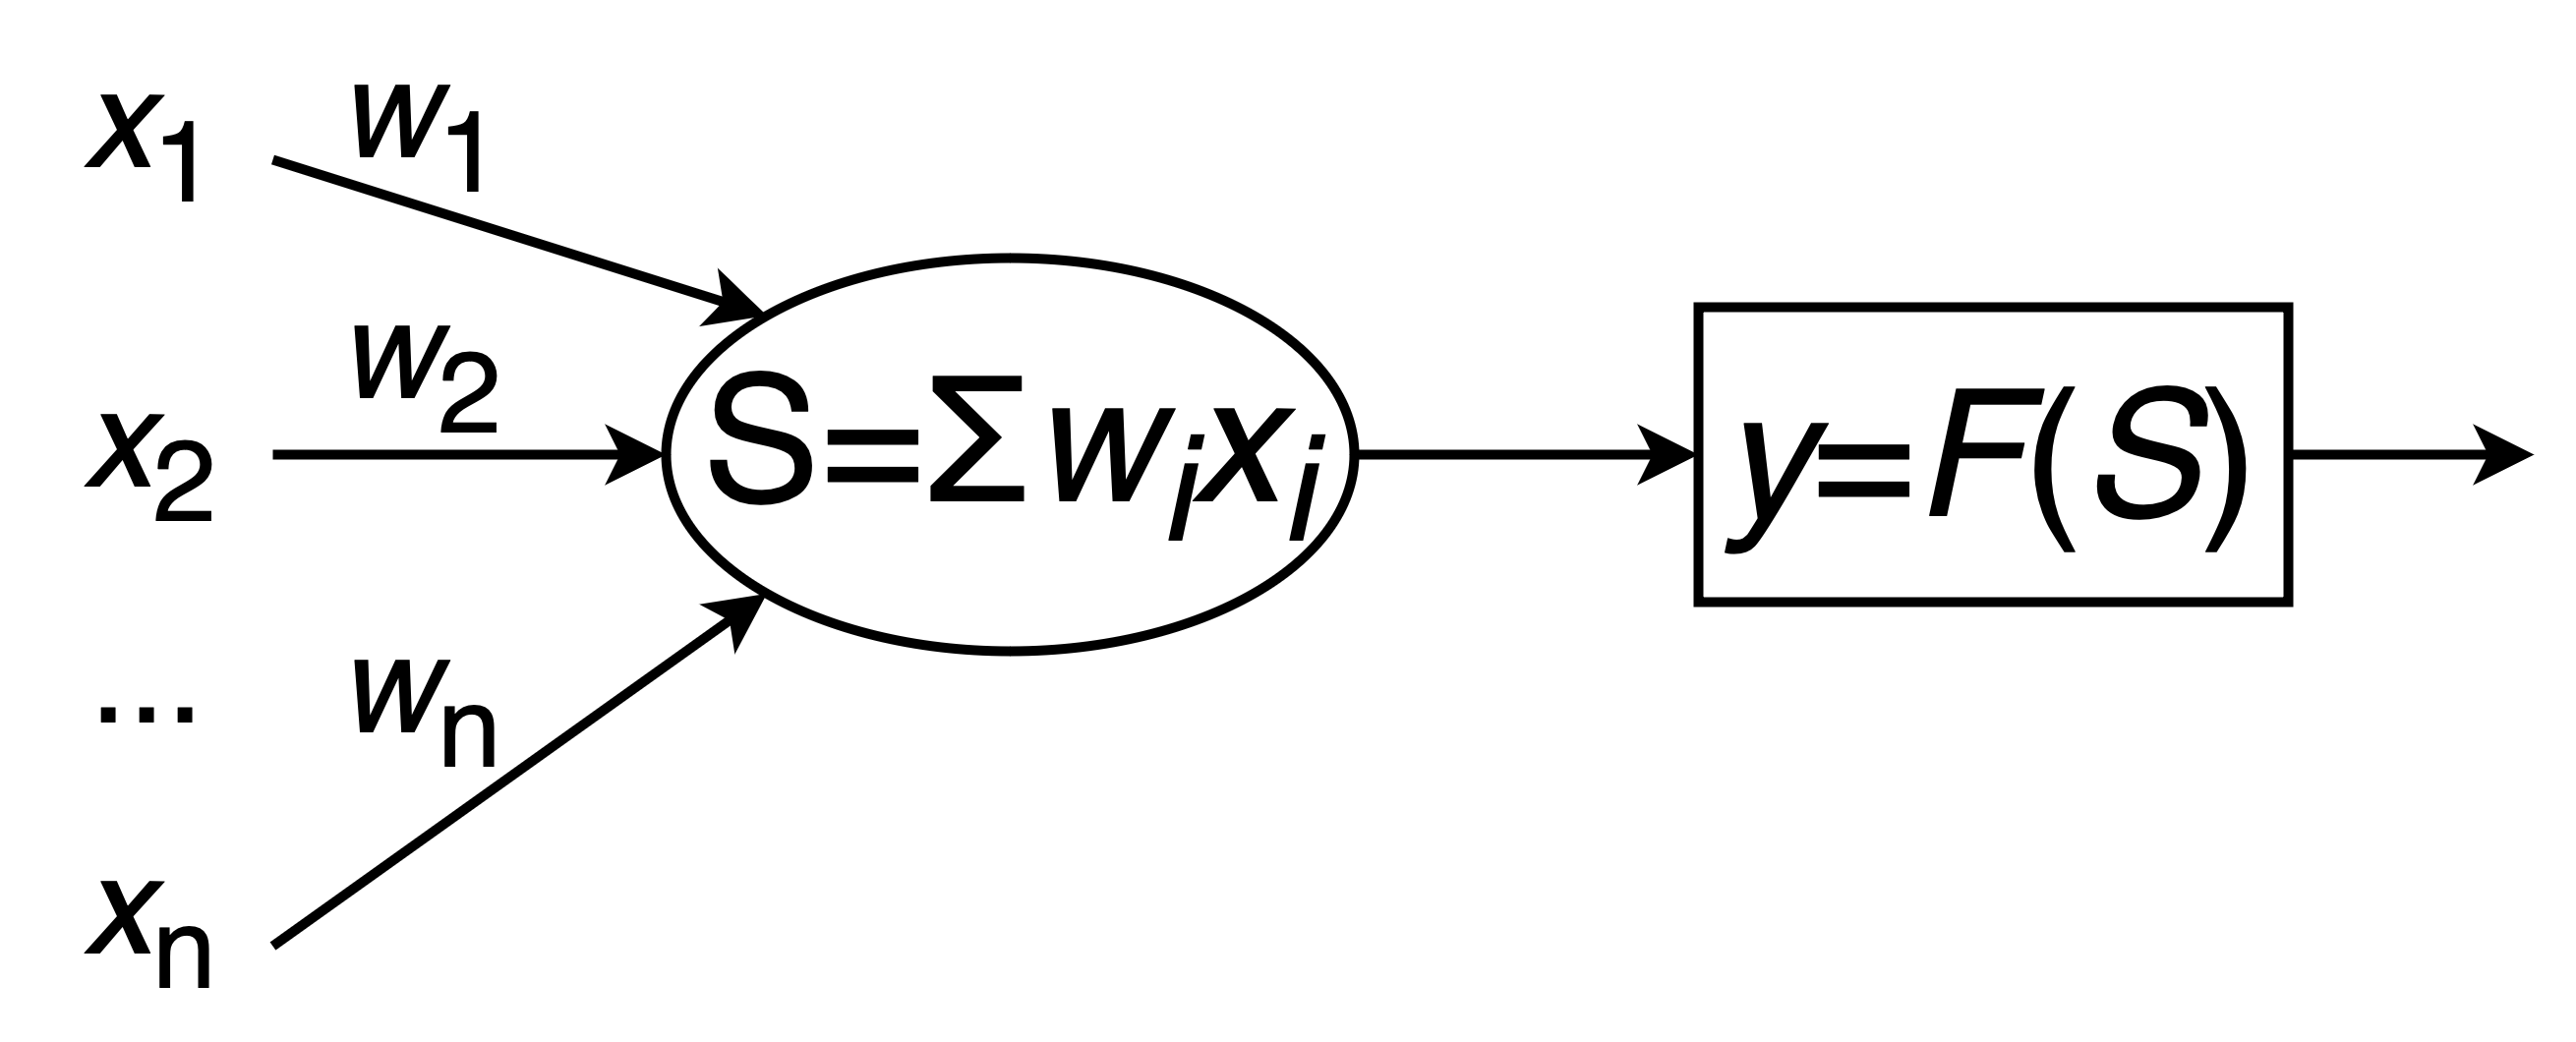
\includegraphics[width=\textwidth]{man-source/images/ch1/pic0-1.png}
  \caption{Модель искусственного нейрона}
  \label{fig:pic0_1}
\end{figure}

Искусственные нейроны могут быть объединены в группы, называемые слоями, по аналогии с биологическими нейронными слоями. Каждый нейрон слоя, обладая независимым набором весовых коэффициентов, получает на вход одинаковый вектор данных $X$ и выполняет его преобразование, формируя отдельную компоненту выходного вектора $Y$, называемого паттерном выходной активности слоя (рис. \ref{fig:pic0_2}). Весовые коэффициенты отдельных нейронов для удобства объединяются в матрицу, которая называется матрицей весовых коэффициентов слоя (или матрицей весов). Слой, имеющий настраиваемые параметры, называется обрабатывающим (в отличие от распределительных слоев, которые являются предваряющими в любой НС и не имеют параметров).

\begin{figure}[H]
  \centering
  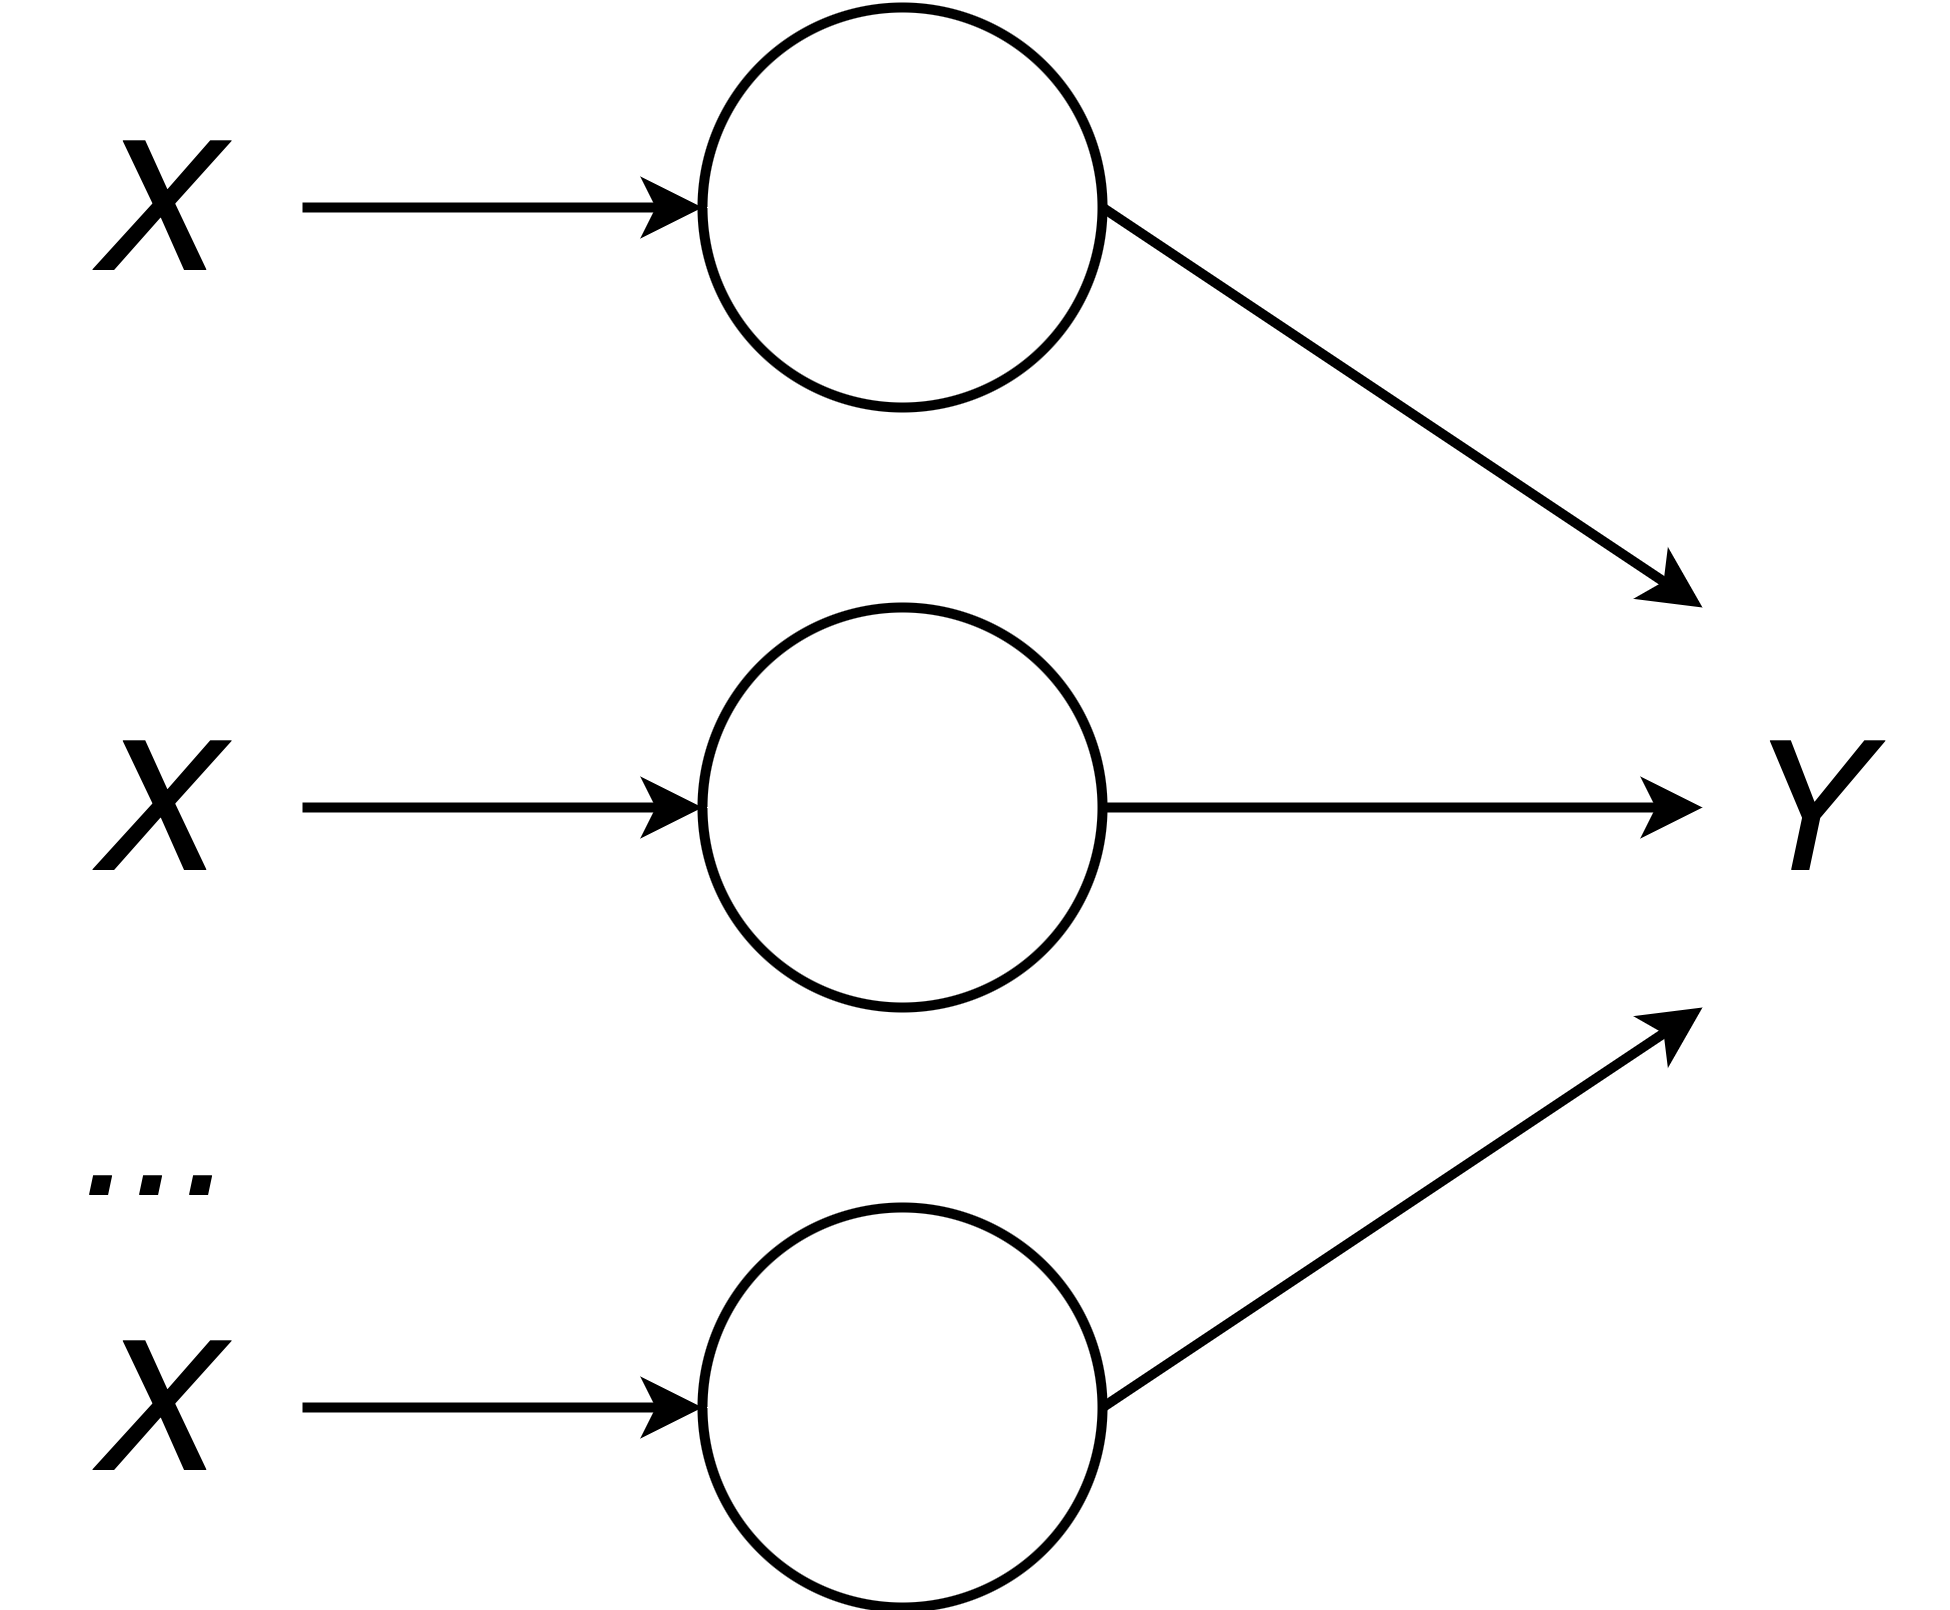
\includegraphics[width=0.6\textwidth]{man-source/images/ch1/pic0-2.png}
  \caption{Слой нейронных элементов}
  \label{fig:pic0_2}
\end{figure}

Наконец, слои нейронных элементов объединяются в последовательности, формируя общую архитектуру нейронной сети (последовательность слоев, их тип, количество нейронов в каждом слое, функцию активации и т.д.). Итоговая модель способна выполнять аппроксимацию любой непрерывной функции с любой точностью после выполнения обучения \cite{Cybenko1989ApproximationBS}. В процессе обучения данные из некоторой выборки подаются на вход сети с целью определения градиентов изменения параметров нейронных элементов. Одна итерация, в ходе которой модели предъявляются все обучающие примеры, называется эпохой. Данная процедура выполняется до тех пор, пока не будет достигнут ответ сети, полученный с желаемой точностью или пока весовые коэффициенты не войдут в некоторое стационарное состояние. 

Искусственные нейронные сети могут быть классифицированы по различным признакам (например, по характеру обучения, по направлению связей, по архитектуре и т.д.). В литературе часто используется классификация по архитектурному признаку. Согласно ей, выделяют \cite{golovko2017}:

\begin{easylistNum}
    & Сети персептронного типа (многослойные персептроны \cite{ivakhnenko1967cybernetics}, рекуррентные (\cite{Elman1990FindingSI}, \cite{Jordan1997SerialOA}), рециркуляционные \cite{Hinton1987LearningRB}, сверточные (\cite{fukushima1980}, \cite{LeCun1989HandwrittenDR}), глубокие);
    & Самоорганизующиеся НС (НС Кохонена \cite{kohonen2001}, сети адаптивного резонанса \cite{Grossberg1987CompetitiveLF});
    & Релаксационные НС (сети Хопфилда \cite{Hopfield1984}, Хэмминга \cite{Lippmann1987} и двунаправленная ассоциативная память \cite{Kosko1988BidirectionalAM});
    & Гибридные НС (сети встречного распространения \cite{HechtNielsen1987}, RBF-сети \cite{Broomhead1988}, нечеткие сети \cite{Jang1997});
    & Нейронные иммунные сети \cite{Golovko2010}.
\end{easylistNum}

В данной работе исследуются глубокие нейронные сети, являющиеся развитием архитектур полносвязных сетей (персептронов) и сверточных нейронных сетей.

В настоящий момент сверточные нейронные сети и глубокие архитектуры на их основе являются доминирующими в области компьютерного зрения \cite{LeCun2015}. В основном это связано с тем, что в подобных задачах используются данные с высокой корреляцией между соседними элементами (для цифровых фотографий и видео в качестве этих значений выступают массивы пикселей), а сверточные слои особенно эффективны при обработке именно таких данных \cite{Emmert2020}.

Сверточные нейросети могут включать как сверточные слои, так и некоторое количество полносвязных слоев (например, это справедливо для моделей классификации, в которых последние слои часто являются полносвязными и представляют классификаторы признаков, извлеченных на начальных сверточных слоях). %Таким образом, исследование и обучение полносвязных архитектур остается актуальной задачей. 

Несмотря на лидирующее положение сверточных сетей, полносвязные архитектуры также успешно применяются для некоторых задач компьютерного зрения (например, при решении задачи трехмерной реконструкции \cite{mildenhall2020nerf}). Далее в работе будет показано, что сверточный слой может быть представлен с помощью разряженного слоя. Таким образом, исследование и обучение полносвязных архитектур остается актуальной задачей. 

Cтрогого определения понятия глубокой нейронной сети не существует, но ее можно определить как искусственную нейронную сеть с архитектурой персептронного типа, имеющую более двух скрытых слоев нейронных элементов.

В общем случае глубокая нейронная сеть (deep neural network -- DNN) представляет собой нейросетевую модель с множеством слоев нейронных элементов. Рассмотрим полносвязную нейросетевую модель -- многослойный персептрон (рисунок~\ref{fig:pic1_1}). Известно, что такая сеть осуществляет глубокое иерархическое преобразование входного пространства образов \cite{n5}. 

\begin{figure}[H]
  \centering
  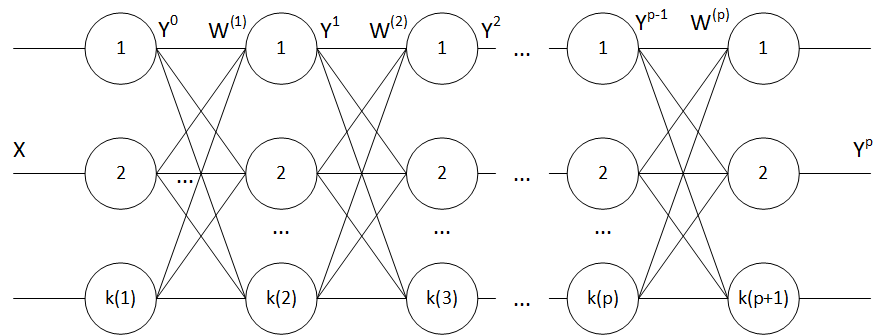
\includegraphics[width=\textwidth]{man-source/images/ch1/pic1-1.png}
  \caption{Глубокая нейронная сеть}
  \label{fig:pic1_1}
\end{figure}

Первый скрытый слой выделяет низкоуровневое пространство признаков входных данных, второй слой определяет пространство признаков более высокого уровня абстракции и т.д. \cite{n3}. 

Выходное значение $j$-го нейрона $k$-го слоя определяется следующим образом:

\begin{equation}
y_j^k=F(S_j^k),
\end{equation}

\begin{equation}
S_j^k=\sum_{i=1} w_{ij}^ky_i^{k-1}+T_j^k,
\end{equation}
где $F(\cdot)$ -- функция активации нейронного элемента \textit{k}-го слоя, $S_j^k$ -- взвешенная сумма $j$-го нейрона $k$-слоя, $w_{ij}^k$ -- весовой коэффициент между $i$-ым нейроном ($k$-1)-го слоя и $j$-м нейроном $k$-го слоя, $T_j^k$ -- пороговое значение $j$-го нейрона $k$-го слоя.

Для первого слоя НС, называемого распределительным, справедливо		
\begin{equation}
y_j^0=x_j.
\end{equation}

В матричном виде выходной вектор $k$-го слоя 

\begin{equation}
Y^k=F(S^k)=F((Y^{k-1})^TW^k+T^k),
\end{equation}
где $W^k$ -- матрица весовых коэффициентов $k$-го слоя, $Y^{k-1}$ -- выходной вектор-столбец ($k$-1)-го слоя, $T^k$ -- вектор пороговых значений нейронов $k$-го слоя.

Если глубокая нейронная сеть используется для классификации образов, то выходные значения сети часто определяются на основе функции активации \textbf{softmax} \cite{golovko2017}: 		

\begin{equation}
y_j^F=softmax(S_j)=\frac{e^{S_j}}{\sum_i e^{S_i}}
\end{equation}
В этом случае значения, получаемые на последнем слое нейронной сети, отражают вероятность принадлежности данного образа к определенному классу.
%Большинство современных архитектур нейросетевых моделей, решающих задачи компьютерного зрения (классификация, идентификация и детекция объектов, аннотирование и генерация изображений и др.) содержат в своем составе сверточные слои. При этом такие модели могут включать как чисто сверточные слои, так и некоторое количество полносвязных слоев. Однако, и те, и другие называются в этом случае сверточными нейронными сетями. Далее будет показано, что сверточный слой может быть представлен с помощью полносвязного. 

%Интенсивность исследований в области нейронных сетей никогда не выражалась однородным течением. Так, зародившись в работах ... в начале 1940 годов, исскуственным нейронным сетям были посвящены концептуальные и важные работы того времени, которые, однако, были забыты после опубликования работы ... в 1969 году. В данной работе был проведен анализ персептронной модели и выявлены его основные ограничения. Данная работа повлияла на развитие теории и, вплоть до ..., теория не развивалась. С предложенным Дж. Хинтоном методом обратного распространения количество работ в этой области стало увеличиваться, однако, интерес к самим моделям по-преждему находился на недостаточном уровне. Так не безосновательно считалось, что обучение нейронных сетей (в частности, персептронных моделей) с более чем двумя скрытыми слоями бесперспективно. Это было главным образом связано с количеством В 2006 году Дж. Хинтоном была предложен иной подход к обучению так называемых глубоких моделей, который ознаменовал начало новой эпохи в развитии теоретических работ в данной области. Развитие вычислительной техники, с другой стороны, ознаменовало новый виток в реализации возможностей обучения и использования подобных моделей.

% Успехи, достигнутые сегодня в этой области, удивляют и дают основания для продолжения исследования возможностей данных моделей и методов их обучения. 

\section{Проблемы обучения глубоких моделей}

Теория нейронных сетей не развивалась равномерно. Нередко причинами приостановок в исследованиях являлось отсутствие доступных на определенный момент времени эффективных методов обучения моделей. 

Начиная с первых моделей ИНС, описанных в работе У. Мак-Каллока и У. Питтса \cite{mcculloch43a} в 1943 году, искусственным нейронным сетям были посвящены концептуальные и важные работы того времени (например, \cite{hebb1949}, \cite{widrow1960}). В 1959 году Ф. Розенблатт предложил модель персептрона \cite{rosenblatt1959}. Однако, после опубликования монографии М. Минского и С. Пайперта <<Персептроны>> в 1969 году \cite{minsky69perceptrons} крупные исследования в этой области были приостановлены. В этой работе был проведен анализ персептронной модели и выявлены ее основные ограничения, в том числе касающиеся невозможности эффективного решения существующими на тот момент моделями некоторых задач (например, задач инвариантного представления образов). %Это повлияло на развитие нейронных сетей и, вплоть до 1985 года, теория не развивалась. 

В конце 1970-х годов произошел очередной всплеск работ, посвященных нейросетевым моделям (например, \cite{Grossberg1976}, \cite{Kohonen1977}).
В 1986 году Д. Румельхартом, Дж. Хинтоном и Р. Вильямсом в работе \cite{rumelhart1986learning} был предложен метод обратного распространения ошибки для обучения многослойных моделей. Результаты, изложенные в данной работе, открыли теоретические возможности для обучения моделей с большим количеством слоев.  Однако, вплоть до середины 2000-х годов сети с количеством слоев три и более широко не применялись, так как считалось, что использование глубоких моделей не дает существенного прироста в эффективности по сравнению с другими подходами. Неэффективность была связана с проблемой <<исчезающего>> градиента. Она проявляется в том, что при обучении глубокой нейронной сети методом обратного распространения ошибки значения градиентов весовых коэффициентов первых слоев сети быстро становятся близкими к нулю, в результате весовые коэффициенты таких слоев практически не изменяются \cite{n5}. Это существенно замедляет процесс обучения, делая невозможным практическое применение подобных моделей по сравнению с другими существовавшими на тот момент времени методами (например, \cite{Corinna1995}).

Тем не менее, проводя аналогии с многоуровневыми нейронными архитектурами в человеческом мозге (в частности, строением вентральной зрительной системы), было понятно, что подобный тип искусственных нейронных сетей обладает полезными свойствами, позволяя формировать многоуровневую иерархию признаков \cite{Behnke2003}.

В 2006 году Джеффри Хинтоном был предложен подход к обучению глубоких моделей, который ознаменовал начало новой эпохи в развитии теоретических работ в данной области \cite{n1}.

В предложенном методе использовался <<жадный>> алгоритм послойного предобучения глубоких нейронных сетей (greedy layer-wise algorithm), основанный на применении ограниченных машин Больцмана, последовательно формируемых и обучаемых из слоев глубокой нейронной сети. 

С этой работы фактически начался новый подъем в исследованиях нейронных сетей, который длится до настоящего времени. За последующие годы в области компьютерного зрения благодаря применению глубоких нейронных сетей удалось значительно улучшить результаты для различных задач, включая классификацию, детекцию, сегментацию объектов на изображении, генерацию текстовых описаний к изображениям, генерацию изображений по текстовым описаниям и т.д.  % Последовавший всплеск количества работ, посвященных обучению и применению глубоких сетей в различных сферах, позволил в течение последующих нескольких лет значительно улучшить первоначальные результаты.

В течение следующих лет сместился основной акцент в исследованиях -- вместо послойного обучения стали применяться методы, позволяющие обучать глубокие нейронные сети, начиная с произвольной начальной инициализации, без использования предобучения (например, стохастический градиентный спуск с использованием функции активации ReLU и ее вариантов). Однако, применение таких подходов не снижает требований к объему обучающей выборки, которая в идеальных теоретических условиях должна быть сравнима с числом настраиваемых параметров модели, поскольку большие модели, обучаемые на малых выборках, с большей вероятностью будут переобучаться. Результатом этого является отличная приспособленность модели к обучающей выборке, но плохая обобщающая способность, т.е. неэффективность сети на тестовых данных. Таким образом, объем используемой обучающей выборки для глубоких нейронных сетей остается по-прежнему критичным фактором для обучения. Даже наличие подходящей по объему выборки не гарантирует успешное завершение обучения, так как подготовка больших моделей может повлечь неприемлемые аппаратные издержки (\cite{alpaca2023}, \cite{alpacagithub}, \cite{zhang2022opt}).

\section{Методы обучения}

Рассмотрим основные методы, применяемые для обучения глубоких нейронных сетей.

Существуют два основных подхода к обучению глубоких нейронных сетей, оба из которых используют предобучение:

\begin{easylistNum}    
    & Обучение с использованием предобучения на большой обучающей выборке и любого оптимизирующего метода для настройки параметров нейронной сети (I тип);
	& Обучение с использованием неконтролируемого предобучения (II тип).
\end{easylistNum}

Предобучение I типа представляет собой обучение модели с использованием метода обратного распространения ошибки \cite{Glorot2011}, некоторого оптимизирующего метода и активационных функций ReLU и ее вариантов в качестве функций активации нейронов \cite{LeCun2015}, а затем дообучение полученной модели для новой выборки (transfer learning). 

Среди основных оптимизирующих методов, применяемых для предобучения I типа, выделяют:

\begin{easylistNum}
	& SGD (стохастический градиентный спуск). В данном методе корректировка настраиваемых параметров ИНС выполняется в направлении, противоположном вектору градиента функции потерь \cite{Haykin2006};
	& Метод Нестерова. Обучение методом стохастического градиентного спуска нередко происходит очень медленно. Импульсный метод позволяет ускорить обучение, особенно в условиях высокой кривизны, небольших, но устойчивых градиентов или зашумленных градиентов. В импульсном методе вычисляется экспоненциально затухающее скользящее среднее прошлых градиентов и продолжается движение в этом направлении. Метод Нестерова является вариантом импульсного алгоритма, в котором градиент вычисляется после применения текущей скорости \cite{Goodfellow2017};
	& AdaGrad: данный метод по отдельности адаптирует скорости обучения всех настраиваемых параметров ИНС, умножая их на коэффициент, обратно пропорциональный квадратному корню из суммы всех прошлых значений квадрата градиента \cite{Duchi2011};
	& RMSProp. Данный метод является модификацией AdaGrad, которая позволяет улучшить его поведение в невыпуклом случае путем изменения способа агрегирования градиента на экспоненциально взвешенное скользящее среднее. Использование экспоненциально взвешенного скользящего среднего гарантирует повышение скорости сходимости после обнаружения выпуклой впадины, как если бы внутри этой впадины алгоритм AdaGrad был инициализирован заново \cite{Goodfellow2017};
	& Adam. Данный метод можно рассматривать как комбинацию RMSProp и AdaGrad \cite{Kingma2014}. Помимо усредненного первого момента, данный метод использует усредненное значение вторых моментов градиентов.
\end{easylistNum}

I тип фактически представляет собой обучение с нуля, которое осуществляется на больших выборках данных с использованием подходящих аппаратных средств. Предобученные таким образом модели могут быть использованы для решения других задач. Таким образом, современный инженер получает в свое распоряжение репозиторий готовых предобученных моделей, которые могут быть дообучены на небольших выборках данных, предназначенных для решения конкретной задачи.

Рассмотрим подробно реализацию предобучения II типа.

Исследование методов предобучения II типа остается актуальной и перспективной задачей, поскольку позволяет существенно сократить объем применяемой обучающей выборки (для малых обучающих выборок позволяет преодолеть переобучение \cite{LeCun2015}) и жесткие требования к используемой аппаратной части.

В общем случае процесс обучения глубоких нейронных сетей с послойным предобучением (предобучением II типа) можно описать последовательностью из двух этапов \cite{n1, n2, n3, n4}: 
\begin{easylistNum}
	& Предобучение нейронной сети методом послойного обучения, начиная с первого слоя  (pre-training). Такое обучение осуществляется неконтролируемо;
	& Настройка синаптических связей всей сети (fine-tuning) при помощи алгоритма обратного распространения ошибки или алгоритма <<бодрствования и сна>> (wake-sleep algorithm) \cite{hinton1995}.
\end{easylistNum}

%Предобучение I типа осуществляется в два этапа . На первом этапе производится предварительная послойная настройка весов нейронной сети. Процедура начинается с первого слоя и выполняется без учителя (неконтролируемо). На втором этапе выполняется <<тонкая>> настройка весов нейронной сети, используя, например, алгоритм обратного распространения.

\textbf{Первый этап} является <<ядром>> всего подхода.
Выделяют два основных подхода к реализации первого этапа (рисунок~\ref{fig:pic1_2}). %Первый -- метод Хинтона, основанный на применении ограниченных машин Больцмана. Второй подход базируется на обучении автоэнкодерных нейронных сетей. 
В обоих этих методах формирование вспомогательных архитектур (RBM, автоэнкодеров) осуществляется из структуры исходной сети. 

\begin{figure}[H]
  \centering
  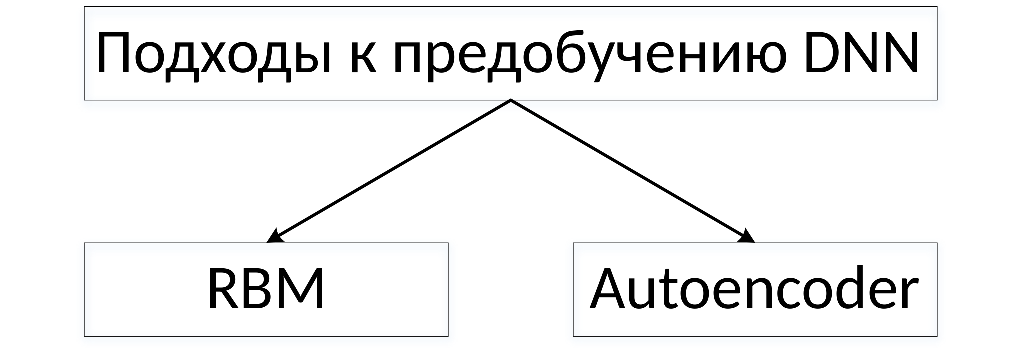
\includegraphics[width=0.7\textwidth]{man-source/images/ch1/pic1-2.pdf}
  \caption{Методы предварительного обучения глубоких нейронных сетей}
  \label{fig:pic1_2}
\end{figure}

Первый подход основывается на представлении каждого слоя нейронной сети в виде ограниченной машины Больцмана (RBM). При использовании второго, автоэнкодерного, подхода, каждый слой  представляется автоассоциативной нейронной сетью.

Рассмотрим каждый из этих подходов подробнее.

% \subsection{Алгоритм обучения ГНС с использованием RBM} \label{subsect1_3_2}
\def\slantfrac#1#2{ \hspace{3pt}\!^{#1}\!\!\hspace{1pt}/
  \hspace{2pt}\!\!_{#2}\!\hspace{3pt}
}

При предобучении ГНС в соответствии с \textbf{первым подходом} осуществляется последовательное конструирование RBM-сетей из параметров скрытых слоев ГНС и их обучение. 

Для понимания подхода рассмотрим модель RBM.

Ограниченная машина Больцмана состоит из двух слоев стохастических бинарных нейронных элементов, которые соединены между собой двунаправленными симметричными связями (рисунок~\ref{fig:pic1_3}). Входной слой нейронных элементов называется видимым (слой $X$), а выходной -- скрытым (слой $Y$). Ограниченная машина Больцмана может генерировать любое дискретное распределение, если используется достаточное количество нейронов скрытого слоя \cite{n5}.

\begin{figure}[H]
  \centering
  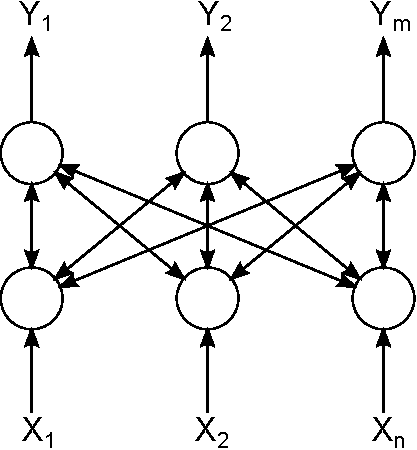
\includegraphics[width=0.4\textwidth]{man-source/images/ch1/pic1-3.pdf}
  \caption{Ограниченная машина Больцмана}
  \label{fig:pic1_3}
\end{figure}	

В данной модели состояния видимых и скрытых нейронов меняются в соответствии с вероятностной версией сигмоидной функции активации:
	
\begin{equation}
	p(y_j\lvert x)=\frac{1}{1+e^{-S_j}},\ S_j=\sum_i^n w_{ij}x_i+T_j
\end{equation}
	
\begin{equation}
	p(x_i\lvert y)=\frac{1}{1+e^{-S_i}},\ S_i=\sum_j^m w_{ij}y_j+T_i
\end{equation}
где $S_i, S_j$ -- взвешенные суммы видимого и скрытого слоев, $T_i, T_j$ -- пороговые элементы видимого и скрытого слоев соответственно.
	
Состояния видимых и скрытых нейронных элементов принимаются независимыми:
	
\begin{equation*}
\begin{aligned}
	P(x \lvert y) = \prod_{i=1}^n P(x_i \lvert y)\\
	P(y \lvert x) = \prod_{j=1}^m P(y_j \lvert x)
\end{aligned}	
\end{equation*}
	
Таким образом, состояния всех нейронных элементов ограниченной машины Больцмана определяются через распределение вероятностей. В RBM нейроны скрытого слоя являются детекторами признаков, которые сохраняют закономерности входных данных. Основная задача обучения состоит в воспроизведении распределения входных данных на основе состояний нейронов скрытого слоя как можно точнее. Для достижения этого применяется процедура CD-\textit{k}. В главе 2 будет подробна описана данная процедура и приведен вывод классических правил обучения RBM. %Это эквивалентно  максимизации функции правдоподобия путем модификации синаптических связей нейронной сети. Покажем основные этапы вывода правил обучения для RBM.

При предобучении ГНС на базе RBM вначале создается RBM-модель из первого скрытого слоя ГНС. Для данной RBM входные данные поступают на видимый слой нейронных элементов и используя CD-$k$ процедуру вычисляются состояния скрытых $P(y \lvert x)$ и видимых нейронов $P(x \lvert y)$. В процессе выполнения данной процедуры в течение заданного количества эпох изменяются весовые коэффициенты и пороговые значения сети RBM, которые затем фиксируются. Следующим берется второй скрытый слой глубокой нейронной сети и конструируется новая RBM. Входными данными для нее являются данные с предыдущего слоя (выходные данные, полученные первой RBM). Выполняется обучение новой модели и процесс продолжается для всех последующих слоев нейронной сети, за исключением, возможно, самого последнего (включение последнего слоя в процесс предобучения зависит от решаемой задачи -- например, для задачи классификации предобучение последнего слоя не требуется, так как он должен обучаться с учителем), как показано на рисунке~\ref{fig:pic1_4}. 

\begin{figure}[H]
  \centering
  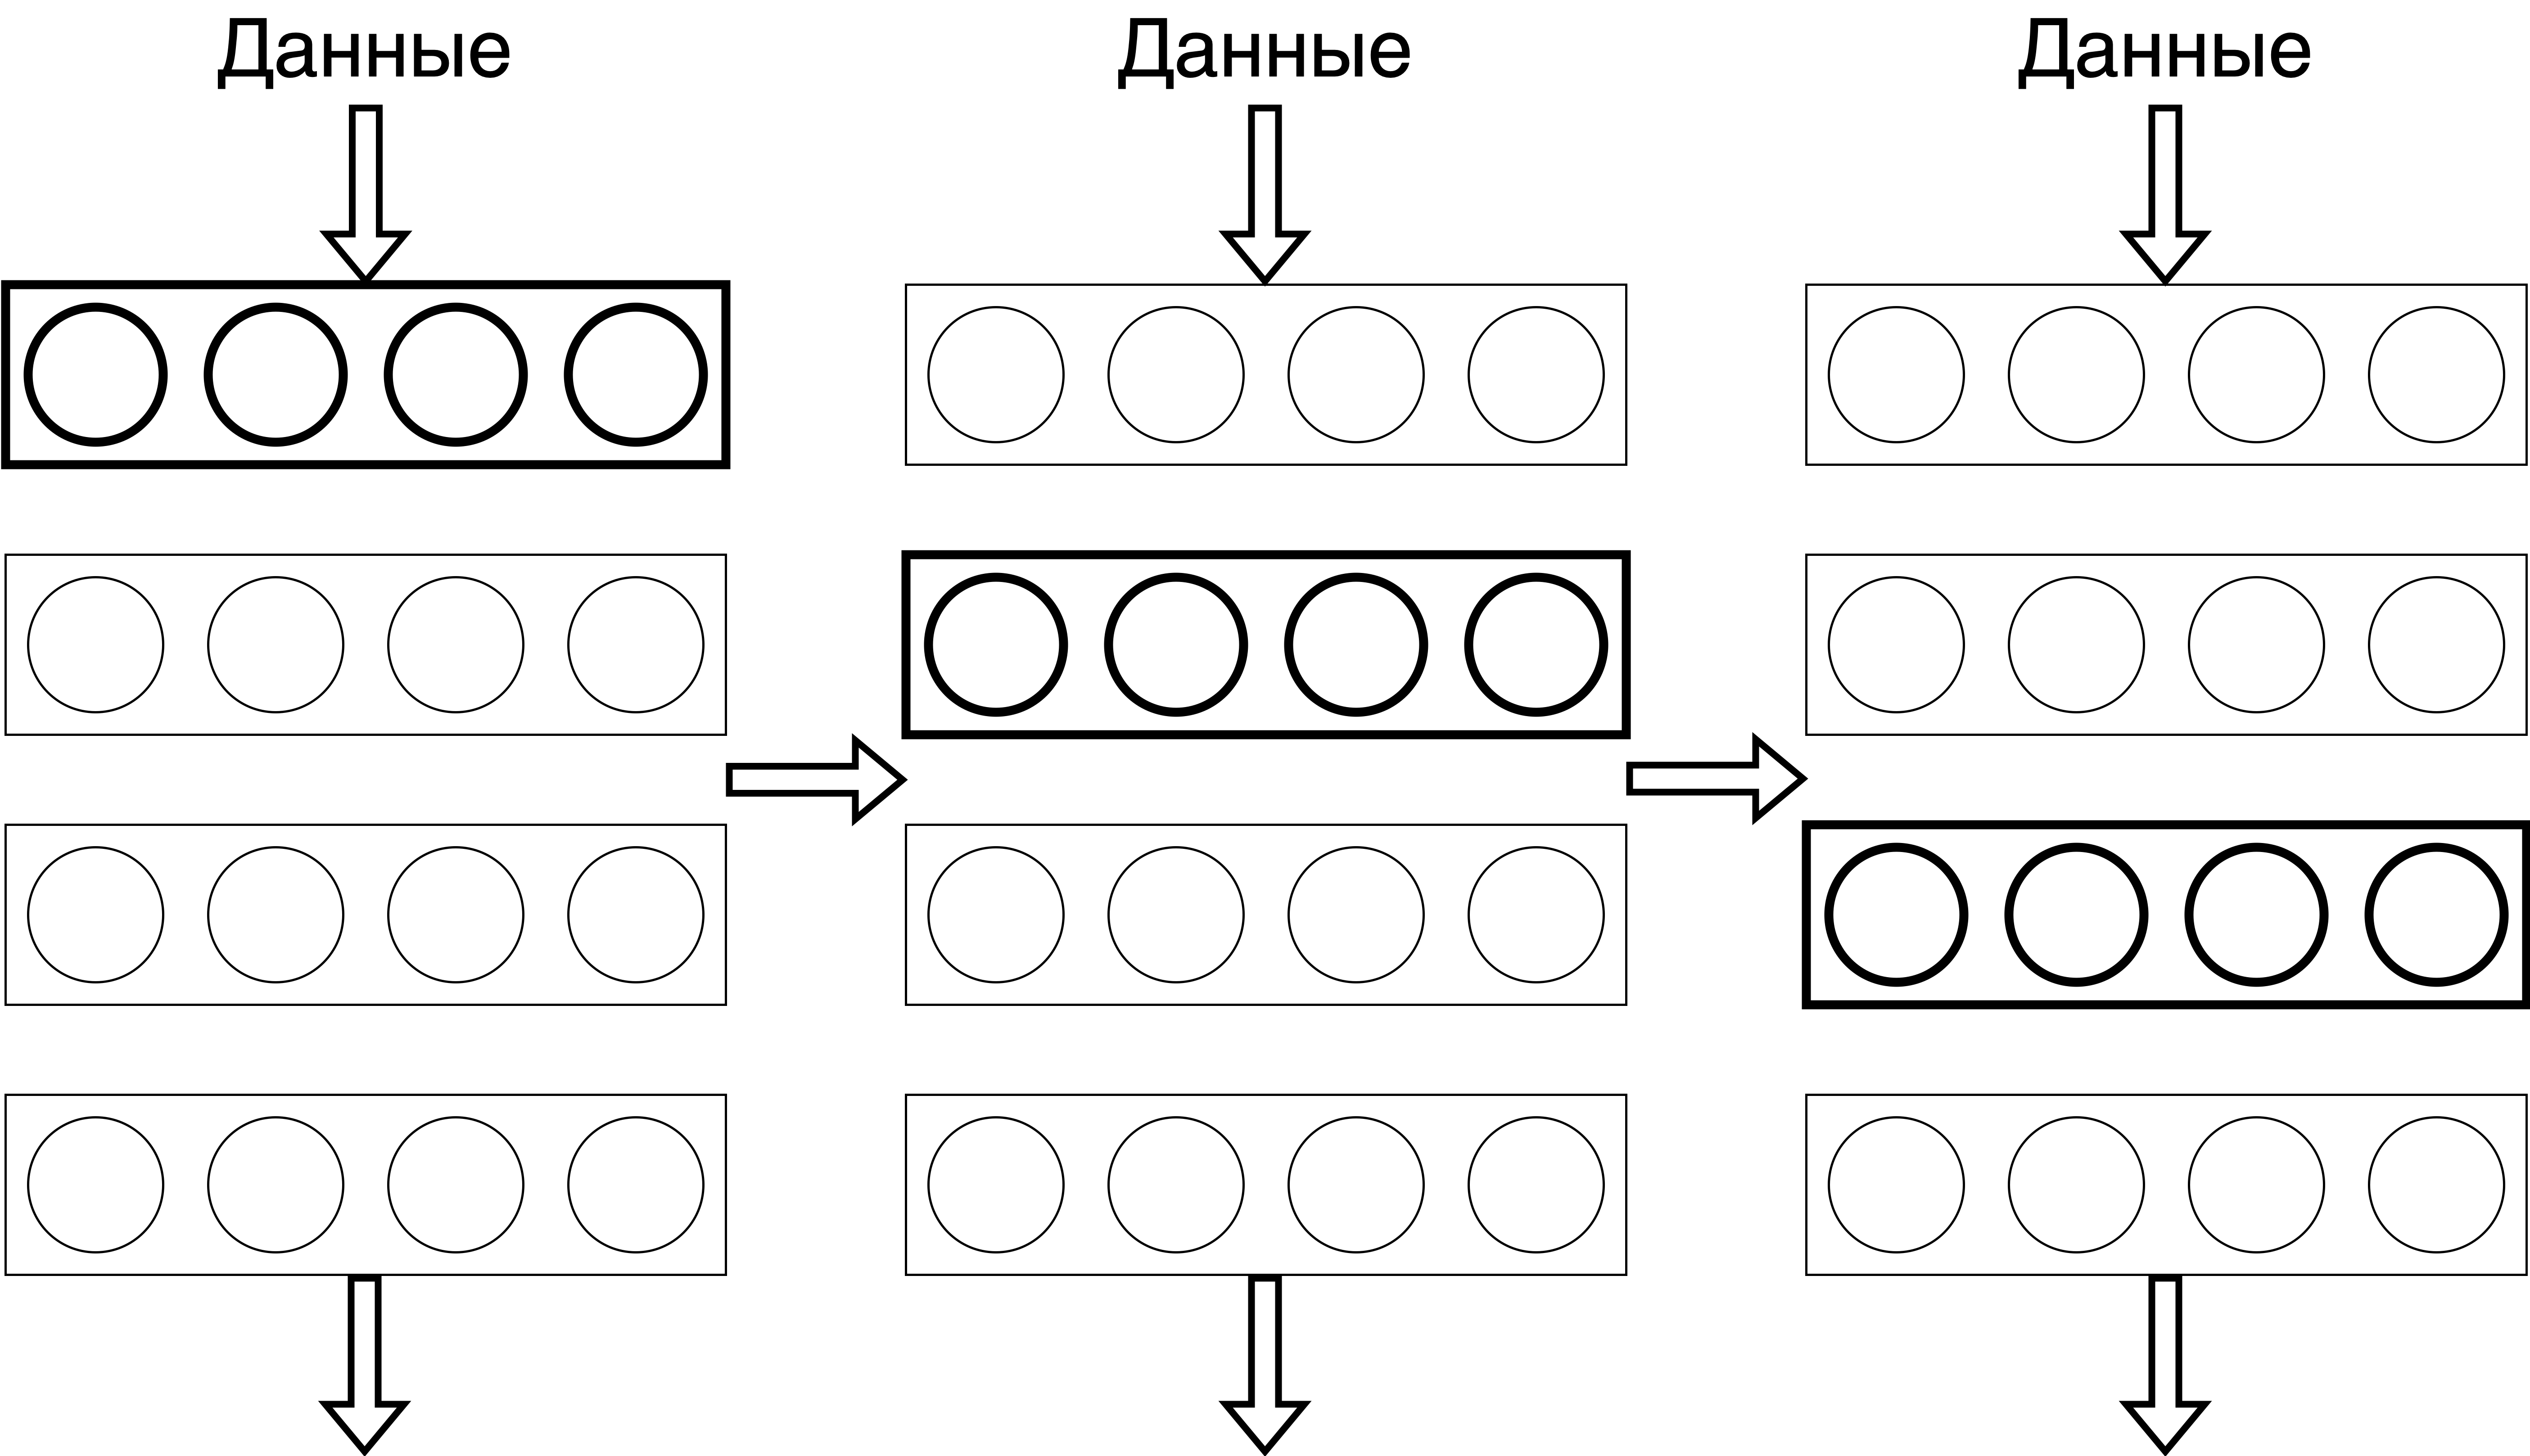
\includegraphics[width=\textwidth]{man-source/images/ch1/pic1-4.png}
  \caption{<<Жадный>> алгоритм послойного обучения}
  \label{fig:pic1_4}
\end{figure}

% \section{Автоэнкодерный метод предобучения} \label{subsect1_3_3}

При предобучении ГНС в соответствии со \textbf{вторым подходом} \cite{n6}, вначале обучается первый слой ГНС как автоассоциативная нейронная сеть с целью минимизации суммарной ошибки реконструкции данных, затем обучается второй слой ГНС и так далее. Для обучения каждого слоя можно использовать алгоритм обратного распространения ошибки. 

%После этого осуществляется точная настройка синаптических связей всей сети (fine tuning), используя алгоритм обратного распространения ошибки. 
	
Рассмотрим персептрон с тремя скрытыми слоями (рисунок \ref{fig:pic1_5}). Тогда в соответствии с автоэнкодерным методом, прежде всего, берутся первые два слоя нейронной сети (1 и 2) и на базе их конструируется автоассоциативная (рециркуляционная) нейронная сеть (1-2-1), то есть добавляется восстанавливающий слой (рисунок \ref{fig:pic1_6}). 

Затем, происходит обучение такой сети, например, при помощи алгоритма обратного распространения ошибки с целью минимизации ошибки реконструкции данных. 
	
\begin{figure}[H]
  \centering
  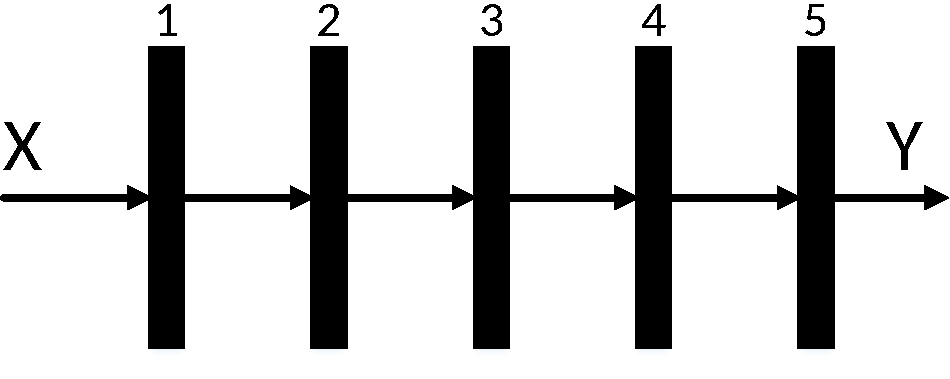
\includegraphics[width=0.7\textwidth]{man-source/images/ch1/pic1-5.pdf}
  \caption{Персептрон с тремя скрытыми слоями}
  \label{fig:pic1_5}
\end{figure}	

\begin{figure}[H]
  \centering
  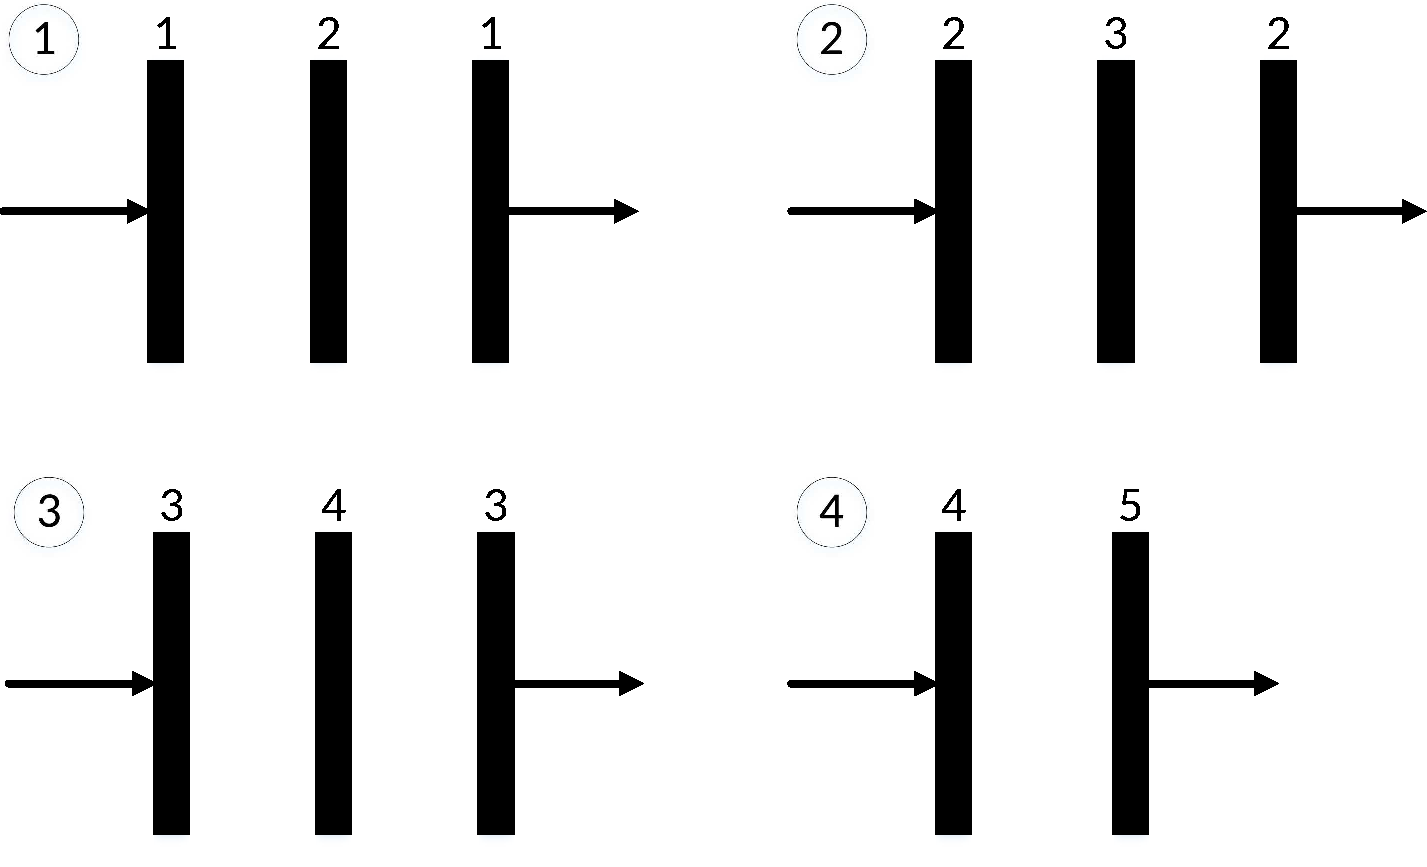
\includegraphics[width=0.7\textwidth]{man-source/images/ch1/pic1-6.pdf}
  \caption{Автоэнкодерный метод обучения}
  \label{fig:pic1_6}
\end{figure}
	
После этого отбрасывается восстанавливающий слой (последний слой) автоассоциативной сети, фиксируются веса скрытого слоя, и конструируется автоассоциативная сеть из следующих двух слоев нейронной сети (2-3-2), которая обучается на основе данных, поступающих с предыдущего (2-го слоя). Процесс продолжается до последнего или предпоследнего слоя, как это схематично изображено на рисунке \ref{fig:pic1_6}. %В результате послойного обучения получается предварительно обученная нейронная сеть. Далее осуществляется точная настройка (fine-tuning) посредством, например, алгоритма обратного распространения ошибки с учителем.
	
Данный процесс можно представить в виде следующего алгоритма:
\begin{easylistNum}
	& Конструируется автоассоциативная сеть с входным слоем $X$, скрытым $Y$ и выходным слоем $X$.
	& Обучается автоассоциативная сеть, например при помощи алгоритма обратного распространения ошибки и фиксируются синаптические связи первого слоя $W_1$ .
	& Берется следующий слой глубокой нейронной сети и снова формируется автоассоциативная сеть аналогичным образом.
	& Используя настроенные синаптические связи предыдущего слоя $W_1$, подаются входные данные на вторую автоассоциативную сеть и она обучается аналогичным образом. В результате получаются весовые коэффициенты второго слоя $W_2$.
	& Процесс продолжается до последнего или предпоследнего слоя нейронной сети.
	%& Берется последний слой нейронной сети и обучается с учителем.
	%& Обучается вся сеть для точной настройки параметров при помощи алгоритма обратного распространения ошибки.
\end{easylistNum}

Для обоих подходов (RBM и автоэнкодерный), с помощью реализации такого неконтролируемого предобучения можно получить приемлемую начальную инициализацию настраиваемых параметров глубокой нейронной сети. 

%\textbf{На втором этапе} производится точная настройка параметров всей сети при помощи алгоритма обратного распространения ошибки или алгоритма <<бодрствования и сна>> (wake-sleep algorithm).
	
% \section{Этап <<тонкой>> настройки глубокой НС}

На \textbf{втором этапе}, иначе называемом этапом <<тонкой настройки>> нейронной сети или fine-tuning, выполняется дообучение всей ГНС некоторым традиционным подходом (например, алгоритмом обратного распространения ошибки или <<бодрствования и сна>>).

Критически важным для этого этапа является начальная инициализация весов и порогов. Если такая инициализация выполнена в ходе предобучения, то сеть начинает процесс <<тонкой настройки>> с <<хороших>> начальных значений, что обуславливает быструю сходимость.

Если же предобучение отсутствует и используется традиционная <<поверхностная>> схема обучения со случайной инициализацией параметров, обучение сети может быстро остановиться и, как результат, приемлемая обобщающая способность не будет достигнута.

В дальнейшем под предобучением будем понимать предобучение I типа, проводимое с использованием RBM-сетей, если не указано иного. 

\section{Критерии минимизации при обучении}

При обучении ГНС (например, на этапе <<тонкой настройки>>, если сеть предобучалась) важно определить критерий минимизации. Наиболее известными и используемыми в настоящий момент функциями ошибок являются функция квадратичной ошибки (SE):

\begin{equation}
	\label{MSE}
	E_{SE} = \frac{1}{2}\sum_{j=1}^{n}(y_j - t_j)^2
\end{equation}
и кросс-энтропийная функция (CE) -- случай мультиклассовой классификации:

\begin{equation}
	\label{CE_multiclass}
	E_{CE_{mult}} = -\sum_{j=1}^{n}t_j\log(y_j)
\end{equation}
где $n$ -- количество нейронных элементов в последнем слое, $y_j$ -- выход нейрона $j$, $t_j$ -- эталонное значение этого нейрона, множитель $\frac{1}{2}$ введен для удобства вычислений.

Формула \ref{MSE} справедлива для одного обучающего примера. Для $L$ обучающих примеров она запишется в следующем виде (MSE -- среднеквадратичная ошибка):

\begin{equation}
	\label{MSE_L}
	E_{MSE} = \frac{1}{2L}\sum_{k=1}^{L}\sum_{j=1}^{n}(y_j^k - t_j^k)^2	
\end{equation}

При обучении автоэнкодеров часто применяется кросс-энтропийная функция, обобщающая двухклассовый случай (\cite{Amaral2013}):

\begin{equation}
	\label{CE}
	E_{CE} = -\sum_{j=1}^n(t_j\log(y_j) + (1-t_j)\log(1-y_j))
\end{equation}

Согласно методу обратного распространения ошибки, для настройки весовых коэффициентов и порогов применяются следующие правила, получаемые в соответствии с методом градиентного спуска:

\begin{equation}
	w_{i-1,i} = w_{i-1, i} - \alpha \frac{\partial E}{\partial w_{i-1, i}}
\end{equation}
\begin{equation}
	T_i = T_i - \alpha \frac{\partial E}{\partial T_i}
\end{equation}
где $w_{i-1,i}$ -- весовые коэффициенты для \textit{i}-го обрабатывающего слоя нейронной сети, \textit{i} изменяется от 1 до \textit{N}, \textit{N} -- количество обрабатывающих слоев нейронной сети, $\alpha$ -- скорость обучения, а соответствующие градиенты находятся по формулам:

\begin{equation}
	\label{weights_delta}
	\frac{\partial E}{\partial w_{i-1, i}} = \frac{\partial E}{\partial S_i} y_{i-1}
\end{equation}
\begin{equation}
	\label{biases_delta}
	\frac{\partial E}{\partial T_i} = \frac{\partial E}{\partial S_i}
\end{equation}
где $\frac{\partial E}{\partial S_i}$ -- частная производная по взвешенной сумме для i-го слоя НС, $y_{i-1}$ -- выход $i-1$-го слоя НС.


Частные производные по взвешенным суммам $S_i$ получаются в соответствии со следующими выражениями:
\begin{equation}
	\label{last_layer_error}
	\frac{\partial E}{\partial S_i} = (y_i - t_i)F'(S_i)
\end{equation}

\begin{equation}
	\label{sum_rec_common}
	\frac{\partial E}{\partial S_{i-1}} = \Bigg(\sum_{i}\frac{\partial E}{\partial S_i}w_{i-1, i}\Bigg)F'(S_{i-1})
\end{equation}
где $F$ -- функция активации нейронных элементов.

Формула \ref{last_layer_error} используется для последнего слоя НС, а формула \ref{sum_rec_common} -- для других слоев, кроме последнего.

Формула \ref{last_layer_error} актуальна для случая, если используется целевая функция $E_{MSE}$. Для случая $E_{CE}$ она будет иметь следующий вид:

\begin{equation}
	\label{last_layer_error_ce}
	\frac{\partial E}{\partial S_i} = \frac{y_i - t_i}{y_i(1-y_i)}F'(S_i)
\end{equation}

В случае использования логистической функции, формула \ref{last_layer_error_ce} упрощается, поскольку в этом случае $F'(S_i)=y_i(1-y_i)$:

\begin{equation}
	\frac{\partial E}{\partial S_i} = y_i - t_i
\end{equation}

Формулы \ref{weights_delta}, \ref{biases_delta} и \ref{sum_rec_common} справедливы как для случая $E_{MSE}$, так и для $E_{CE}$.

Для $E_{CE_{mult}}$ эти формулы справедливы для функции активации \textbf{softmax} на последнем слое нейронной сети. Покажем это.

Имеем

\begin{equation}
	\label{common_E}
	\frac{\partial E_{CE_{mult}}}{\partial S_i} = \sum_{k=1}^{n} \frac{\partial E_{CE_{mult}}}{\partial y_k}\frac{\partial y_k}{\partial S_i} = \frac{\partial E_{CE_{mult}}}{\partial y_i}\frac{\partial y_i}{\partial S_i} + \sum_{k\neq i}\frac{\partial E_{CE_{mult}}}{\partial y_k}\frac{\partial y_k}{\partial S_i}
\end{equation}

Очевидно, 
\begin{equation}
\label{part_deriv_y}
\frac{\partial E_{CE_{mult}}}{\partial y_i} = -\frac{t_i}{y_i}
\end{equation}

Учитывая, что
\begin{equation}
	y_i = \frac{e^{S_i}}{\sum_{k=1}^{n} e^{S_k}}
\end{equation}
где $i$ -- индекс последнего слоя сети, $S_i$ -- соответствующая взвешенная сумма, найдем значения частной производной $\frac{\partial y_i}{\partial S_k}$.
\begin{easylistNum}
	& Случай $i = k$
	\begin{multline}
		\label{part1_deriv_S}
		\frac{\partial y_i}{\partial S_i} = \frac{e^{S_i}\sum e^{S_k} - e^{2S_i}}{(\sum e^{S_k})^2} = \\ = \frac{e^{S_i}\sum e^{S_k}}{(\sum e^{S_k})^2}-\frac{e^{2S_i}}{(\sum e^{S_k})^2}=y_i - y_i^2 = y_i(1-y_i)
	\end{multline}
	& $i \neq k$
	\begin{equation}
		\label{part2_deriv_S}
		\frac{\partial y_k}{\partial S_i} = -e^{S_k}\Big(\sum e^{S_i}\Big)^{-2}e^{S_i} = -y_ky_i
	\end{equation}
\end{easylistNum}

Подставляя полученные выражения \ref{part1_deriv_S}, \ref{part2_deriv_S} и \ref{part_deriv_y} в \ref{common_E}, получим
\begin{equation}
	\frac{\partial E_{CE_{mult}}}{\partial S_i} = -t_i(1-y_i) + \sum_{k\neq i}t_ky_i = -t_i + y_i\sum_{k=1}^{n}t_k = y_i - t_i
\end{equation}

\section{Выводы}

\begin{easylistNum}
    & Дано описание основных понятий теории искусственных нейронных сетей, приведена классификация моделей ИНС.
    & Сформулирована проблема обучения глубоких нейронных сетей, обоснована ее актуальность. Приведены предпосылки развития методов обучения глубоких нейронных сетей.  
    & Рассмотрены существующие методы обучения глубоких нейронных сетей.
    & Описаны основные этапы обучения ГНС с использованием неконтролирумого предобучения, включающие в себя предобучение ГНС и <<тонкую настройку>> модели.
    & Описаны основные подходы к осуществлению неконтролируемого предобучения ГНС, базирующиеся на использовании ограниченных машин Больцмана и автоассоциативных нейронных сетей.
	& Рассмотрены основные критерии минимизации, которые применяются при обучении нейронных сетей, а также дано описание метода обратного распространения ошибки и рассмотрены правила его реализации для различных целевых критериев.
    %& Рассмотрены основные методы неконтролируемого предобучения, приведены основные этапы их осуществления
    %& Рассмотрена теоретическая база, лежащая в основе вывода правил обучения ограниченных машин Больцмана, используемых в свою очередь в качестве одной из базовых моделей при предобучении глубоких нейронных сетей.
    %& Описан этап <<тонкой>> настройки глубокой нейронной сети, позволяющий осуществлять настройку параметров слоев глубокой модели, обучение которых не проводилось на этапе предобучения, а также более точно реконфигурировать параметры слоев, обучавшихся на первом этапе.
\end{easylistNum}

% Согласно классическому определению интеллектуальной системы \cite{AIDictionary1992}, в ее составе выделяются такие ключевые компоненты, как база знаний, решатель задач и интеллектуальный интерфейс. В рамках данной диссертационной работы будем говорить о таком классе решателей, как \textbf{\textit{объединенный решатель задач}}. 

% Будем считать, что объединенный решатель задач, в отличие от решателя задач вообще, в общем случае решает задачи, связанные с:

% \begin{easylist}
% & обеспечением основного функционала системы (решение явно сформулированных задач по требованию);
% & обеспечением корректности и оптимизацией работы системы (перманентно на протяжении жизненного цикла системы);
% & обеспечением автоматизации развития интеллектуальной системы.
% \end{easylist}

% Рассмотрим более подробно, какие именно задачи могут входить в каждый из перечисленных классов.
% Современная интеллектуальная система в общем случае имеет в своем составе следующие подсистемы \cite{Golenkov2014b}:

% \begin{easylist}
% & предметная (основная) подсистема;
% &	интеллектуальный пользовательский интерфейс;
% &	интеллектуальная подсистемы адаптивного управления диалогом с конечным пользователем;
% &	интеллектуальная help-система для информационного обслуживания и обучения конечных пользователей предметной подсистемы, которые, начиная работать с системой, не обязаны иметь сразу высокую квалификацию;
% &	интеллектуальная подсистема управления проектированием интеллектуальной системы, которая координирует деятельность разработчиков предметной подсистемы;
% &	интеллектуальная подсистема управления информационной безопасностью предметной подсистемы.
% \end{easylist}

% В случае интеллектуальной системы, ориентированной не только на взаимодействие с конечным пользователем, но и способной автономно работать в условиях, имеющих высокий уровень непредсказуемости (например, в космосе или других условиях, не пригодных для работы в них человека), в ней должны быть также предусмотрены возможности принятия решений в условиях неопределенности; анализа сигналов, поступающих с различных датчиков, в том числе, средства анализа изображений; анализа последствий собственной деятельности с возможностью автоматической корректировки последующих актов этой деятельности; прогнозирования состояния окружающей среды на основе собранных данных и т. д.

% Задачей всех перечисленных компонентов является не только обеспечение основной функциональности системы, т. е. возможности решать задачи, сформулированные конечным пользователем, но и обеспечение работоспособности самой системы и ее эффективности. Задачи второго типа не всегда явно сформулированы и соответствуют процессам, перманентно выполняющимся на протяжении всего времени работы интеллектуальной системы. К такого рода процессам можно отнести, например, выявление и сборку информационного мусора, оптимизацию базы знаний и т. д. Выполнение некоторых из указанных процессов необходимо для функционирования самой системы и с их прекращением работа системы также прекратится. В особенности это важно в случае автономной системы, для которой важнейшими задачами являются поиск источников энергии, избегание опасных ситуаций во внешней среде и т. д. Таким образом, говоря в рамках данной работы о решении задач, будем подразумевать не только решение задач, инициированных пользователем, но и задач других классов, рассмотренных выше. При этом предполагается, что каждая задача может представлять собой как процедурную спецификацию соответствующего действия, так и декларативную или смешанную.

% Каждая перечисленная подсистема, в свою очередь, состоит из собственной базы знаний, решателя задач и пользовательского интерфейса.

% Приведенный список подсистем отражает необходимость использования в рамках одной и той же системы самых разнообразных моделей решения задач, при этом при решении одной и той же задачи могут одновременно использоваться несколько моделей решения задач. Будем называть решатель задач, способный обеспечить согласованное использование различных моделей решения задач при решении одной и той же комплексной задачи, \textbf{\textit{гибридным решателем задач}}. В рамках данной диссертационной работы основное внимание будет уделено гибридным решателям задач, в частности, принципам, обеспечивающим возможность согласованного использования различных моделей решения задач в рамках одного решателя при решении комплексных задач.

% \bigskip
% Существующее многообразие подходов к решению задач в компьютерных системах можно разделить на два класса:
% \begin{easylist}
% & \textbf{решение задач с использованием хранимых программ.} В данном случае предполагается, что в системе заранее присутствует программа решения задачи заданного класса и решение сводится к поиску такой программы и интерпретации ее на заданных входных данных. К системам, ориентированным на такой подход к решению задач, относятся в том числе системы, использующие:
% && программы, написанные на языках программирования, относящихся как к императивной, так и к декларативной парадигме, в том числе логических и функциональных \cite{Pratt2002};
% && реализации генетических алгоритмов \cite{Gladkov2006,Emelyanov2003};
% && нейросетевые модели обработки знаний \cite{Berkinblit1993,Golovko2001,Gorban1996}.

% Следует отметить, что даже в случае использования хранимой программы решение задачи далеко не всегда тривиально, поскольку, во-первых, требуется найти такую хранимую программу на основе некоторой спецификации, во-вторых, обеспечить ее интерпретацию;

% & \textbf{решение задач в условиях, когда программа решения не известна.} В этом случае предполагается, что в системе необязательно присутствует готовая программа решения для класса задач, которому принадлежит некоторая сформулированная задача, подлежащая решению. В связи с этим необходимо применять дополнительные методы поиска путей решения задачи, не рассчитанные на какой-либо узкий класс задач (например, разбиение задачи на подзадачи, методы поиска решений в глубину и ширину, метод случайного поиска решения и метод проб и ошибок, метод деления пополам и др.), а также различные модели логического вывода (классические дедуктивные \cite{Vagin2008}, индуктивные \cite{Khulick2001,Polya1975}, абдуктивные \cite{Vagin2008}; модели, основанные на нечетких логиках \cite{Batyrshin2001,Demenkov2005,Pospelov1989}, логике умолчаний \cite{Reiter1980}, темпоральной логике \cite{Eremeev1997}, и многие другие).
% \end{easylist}

% Подробный обзор решателей задач, разработанных в период до 1982 г., таких как GPS, STRIPS, QA3, ПРИЗ \cite{Kachro1988}, ППР приведен в книге \cite{Ephymov1982}. Среди современных работ, исследующих вопросы применения моделей решения задач, не ориентированных на конкретную предметную область, можно выделить \cite{Raghovsky2011}.

% Среди наиболее заметных представителей класса интеллектуальных решателей задач, разработанных в более поздний период, можно отметить:
% \begin{easylist}
% &	\textbf{Компьютерный решатель математических задач}

% Указанный программный комплекс разработан А. С. Подколзиным и способен решать задачи уровня конкурсных экзаменов по математике для поступающих в вузы. Система работает с символьной записью задач и ориентируется на использование для решения задачи операций, схожих с теми, что использует человек. Решение можно оформить в протокол, пригодный для подачи прямо в соответствующую экзаменационную комиссию. По словам авторов, решатель справляется с 90 \% задач из указанной предметной области, что соответствует хорошей оценке на экзаменах. Автором системы разработан специальный язык (и компилятор для него), описывающий приемы решения и последовательность их применения, систему распознавания проблемной ситуации, определяющую целесообразность применения тех или иных приемов \cite{Podkholzyn2008}.
% &	\textbf{Решатель задач по планиметрии НИЦ ЭВТ}

% В московском Научно-исследовательском центре электронной вычислительной техники активно ведется разработка средств автоматического решения задач по планиметрии, что отражается регулярными публикациями по данной теме, например \cite{Khurbatov2016}. Разработанные средства способны не только решить поставленную задачу (получить ответ), но и объяснить ход решения, а также отобразить условие задачи и ход решения на чертеже. Для описания условий задачи и способов их решения используется онтологический подход.
% &	\textbf{Системы компьютерной алгебры}

% В настоящее время на рынке наиболее популярны такие системы компьютерной алгебры, как Maple, MathCAD, а также семейство продуктов компании Wolfram Research. Кроме указанных программных комплексов интерес представляет онлайн-сервис Wolpfram Alpha \cite{WolframAlpha}, также построенный на основе разработок компании Wolfram Research. Указанные программные комплексы обладают мощной функциональностью как для проведения различного рода вычислений и экспериментов, так и для построения на их основе систем различного назначения, например обучающих. Подробно возможности применения систем данного семейства рассмотрены, например, в работе \cite{Taranchuk2015}.

% &	\textbf{Программный комплекс <<УДАВ>>}

% В программном комплексе «УДАВ» реализован метод логического вывода, который базируется на миварной логической сети правил и представляет, согласно работам авторов, возможность активного обучения логического вывода, управляемого потоком данных, со снижением вычислительной сложности с N! (факториал) до линейной. «УДАВ» работает со знаниями, представленными в виде продукционных правил и процедур. Однако при всех перечисленных достоинствах указанного метода он представляет собой один из возможных методов решения задач определенных классов и сам по себе не решает проблему интеграции различных моделей решения задач в рамках одной интеллектуальной системы \cite{Vladimirov2010}.

% \end{easylist}

% Однако при всем многообразии решаемых рассмотренными системами задач множество классов задач ограничивается имеющимся в системе набором жестко заданных приемов и алгоритмов решения задач, явно используемых при решении той или иной задачи.

% Рассмотрим более подробно один из примеров комплексных задач, перечисленных выше, связанный с автоматизацией производства.

% В рамках системы комплексной автоматизации производства условно можно выделить следующие уровни автоматизации:
% \begin{easylist}

% &	автоматизация собственно процесса производства продукта на всех этапах, от получения и оценки сырья или исходного материала до фасовки и доставки товара конечному потребителю;
% &	автоматизация управления процессом производства, т. е. автоматизация внесения изменений в процесс производства, например, изменение объемов партии, номенклатуры или свойств изготовляемого продукта и т. д.;
% &	автоматизация контроля выполнения процесса производства, предполагающая использование различных способов анализа текущей ситуации, а также механизмы выявления, классификации и устранения нештатных ситуаций вплоть до полного устранения нештатной ситуации без вмешательства оператора.

% \end{easylist}

% На рисунке~\ref{fig:pic1_1} изображена условная схема системы автоматизации процесса производства, показывающая, применение каких из перечисленных выше моделей решения задач актуально в каждой из подсистем такой системы.

% \begin{figure}[H]
%   \center
%   \includegraphics[width=\linewidth]{man-source/images/ch1/pic1_1.pdf}
%   \caption{Упрощенная схема системы комплексной автоматизации производства} 
%     \label{fig:pic1_1}
% \end{figure}

% На рисунке~\ref{fig:pic1_2} более детально показана условная схема подсистемы обработки нештатных ситуаций.

% \begin{figure}[H]
%   \center
%   \includegraphics[width=0.65\linewidth]{man-source/images/ch1/pic1_2.pdf}
%   \caption{Упрощенная схема подсистемы обработки нештатных ситуаций} 
%     \label{fig:pic1_2}
% \end{figure}

% Приведенный пример показывает, что построение такой системы комплексной автоматизации невозможно без обеспечения согласованного использования различных видов знаний и моделей решения задач в рамках одной системы при решении одной и той же комплексной задачи. Кроме того, становится актуальной задача поддержки такой системы в состоянии, соответствующем текущему уровню развития технологий производства, дополнения ее более совершенными моделями и методами решения задач. При этом очевидно, что подобная реконфигурация системы должна осуществляться \underline{непосредственно в процессе эксплуатации системы}, а не требовать каждый раз полной остановки всего производства или отдельных его частей.

% Актуальность проблемы интеграции результатов, полученных в рамках различных научных школ и направлений в области искусственного интеллекта, в том числе обработки знаний и решения задач, подтверждается, например, работой \cite{Khakhalyn2008}, а также наличием ежегодных международных конференций Artificial General Intelligence \cite{AGI2017}, одной из целей которых является решение указанной проблемы.

% Сказанное выше позволяет сформулировать требования к решателю задач интеллектуальной системы, способной решать комплексные задачи (гибридному решателю задач):
% \begin{easylist}
% &	в каждый момент времени решатель должен обеспечивать решение задач из оговоренного класса за оговоренное время, при этом результат решения задачи должен удовлетворять некоторым известным требованиям. Другими словами, как и в случае современных компьютерных систем, корректность результатов решения задач на этапе разработки системы должна верифицироваться специальными методами, в том числе для этого могут быть использованы такие современные подходы, как unit-тестирование, тестирование методом «черного ящика» и др. \cite{Kaner1999}. Более детально рассмотрим некоторые положения, уточняющие сформулированное требование:

% &&	для явно сформулированных задач система всегда должна давать какой-либо ответ за оговоренное время, при этом ответ может быть отрицательным (система не смогла решить поставленную задачу), возможно, с объяснением причин, по которым решение в текущий момент оказалось невозможным. Одним из факторов безуспешности решения является выход за рамки установленного промежутка времени;
% &&	если явно сформулированная задача решена, то все информационные процессы, направленные на ее решение, должны быть уничтожены. Особенно актуальным данное требование становится в ситуации, когда для решения одной и той же задачи параллельно используются сразу несколько подходов и заранее неизвестно, какой из них приведет к результату раньше других;
% &&	после решения задачи вся временная информация, сгенерированная в процессе решения этой задачи и имеющая ценность только в контексте решения указанной задачи, должна быть удалена из памяти;

% & \textit{\textbf{гибридный решатель}} должен обеспечивать возможность \textbf{согласованного использования различных моделей решения задач} при решении одной и той же комплексной задачи в случае необходимости;

% & решатель должен быть легко \textbf{модифицируемым}, т. е. трудоемкость внесения изменений в уже разработанный решатель должна быть минимальна. Путями повышения модифицируемости решателя являются обеспечение локальности вносимых изменений, в том числе -- за счет стратификации решателя на независимые уровни и обеспечение максимальной независимости компонентов решателя друг от друга, а также наличие готовых компонентов, которые могут быть встроены в решатель при необходимости. При этом внесение изменений должно осуществляться \underline{непосредственно в процессе эксплуатации системы};

% & для того чтобы интеллектуальная система имела возможность анализировать и оптимизировать имеющийся решатель задач, интегрировать в его состав новые компоненты (в том числе самостоятельно), оценивать важность тех или иных компонентов и применимость их для решения той или иной задачи, спецификация решателя должна быть описана языком, понятным системе, например, при помощи тех же средств, что и обрабатываемые знания. Возможность интеллектуальной системы анализировать (верифицировать, корректировать, оптимизировать) собственные компоненты будем называть \textbf{рефлексивностью};

% & дополнительным требованием, предъявляемым к \underline{объединенному} решателю задач по отношению к решателю задач вообще, является его \textbf{полнота} (целостность, комплексность), т. е. такой решатель должен обеспечивать всю функциональность системы, обеспечивать решение всех задач, как связанных с непосредственным назначением системы, так и обеспечивающих эффективность ее работы. Таким образом, например, решатель, реализующий какой-либо вариант логического вывода, не может считаться объединенным, поскольку для использования системы, содержащей такой решатель, необходимо иметь хотя бы базовые средства информационного поиска, позволяющие локализовать полученный ответ, а также средства, обеспечивающие трансляцию вопроса от пользователя в систему и ответа от системы пользователю.
% \end{easylist}

% Поскольку данная диссертационная работа посвящена разработке комплекса моделей, методики и средств, обеспечивающего построение и модификацию решателей задач, то сформулируем также требования, предъявляемые к технологиям разработки таких решателей:

% \begin{easylist}
% &	\textbf{комплексность и совместимость,} т. е. возможность реализовать с помощью такой технологии различные модели решения задач в унифицированном виде, позволяющем обеспечить их совместимость в рамках одного гибридного решателя при решении комплексных задач;
% &	\textbf{снижение сроков и трудоемкости построения решателей} за счет:
% &&	обеспечения согласованности деятельности коллектива разработчиков;
% &&	возможности использования готовых компонентов различной сложности и наличия библиотек таких компонентов, включающих средства спецификации компонентов и поиска компонентов на основе спецификации;
% &&	автоматизации деятельности разработчиков;
% &&	возможности выделения в рамках разрабатываемого решателя достаточно независимых компонентов, разработка которых может вестись отдельно друг от друга при условии, что трудоемкость согласования разработанных таким образом компонентов будет минимальной;
% &&	наличия в технологии средств информационной поддержки разработчиков, в том числе средств обучения квалификации;
% &	обеспечение \textbf{модифицируемости} решателей задач, разработанных с использованием данной технологии, непосредственно в процессе эксплуатации системы, т. е. удовлетворение второго из предъявленных выше требований к решателям;
% &	быстрая \textbf{эволюционируемость самой технологии}, предполагающая в том числе наличие средств автоматизации приведения в соответствие текущему состоянию технологии уже разработанных с ее использованием решателей;
% &	\textbf{снижение требований к разработчикам} решателей задач, которое обеспечивается рассмотренными выше средствами снижения сроков и трудоемкости построения решателей, в частности, наличием развитых средств информационной поддержки разработчиков.

% \end{easylist}

% Таким образом, разработка моделей, методики и средств построения и модификации гибридных решателей задач предполагает удовлетворение перечисленных выше требований.

% \newpage
% \section[Проблемы в области построения гибридных\\ решателей задач]{Проблемы в области построения гибридных решателей задач}

% Несмотря на то что в настоящее время существует большое число моделей решения задач, многие из которых реализованы и успешно используются на практике в различных системах, остается актуальной проблема низкой согласованности принципов, лежащих в основе реализации таких моделей, и отсутствия единой унифицированной основы для реализации и интеграции различных моделей, что приводит к тому, что:

% \begin{easylist}
% &	затруднена возможность одновременного использования различных моделей решения задач в рамках одной системы при решении одной и той же комплексной задачи; практически невозможно комбинировать различные модели с целью решения задачи, для которой априори отсутствует алгоритм ее решения;
% &	практически невозможно использовать технические решения, реализованные в одной системе, в других системах, т. е. возможности использования компонентного подхода при построении решателей задач сильно ограничены. Как следствие, велико количество дублирований аналогичных решений в разных системах;
% &	фактически отсутствуют комплексные методики и средства построения решателей задач, которые бы обеспечивали возможность проектирования, реализации и отладки решателей различного вида.

% \end{easylist}

% Следствиями указанных проблем являются:

% \begin{easylist}
% &	высокая трудоемкость разработки каждого решателя, увеличение сроков их разработки, а значит, и увеличение затрат на разработку и поддержку соответствующих интеллектуальных систем;
% &	высокая трудоемкость внесения изменений в уже разработанные решатели, т. е. отсутствует или сильно затруднена возможность дополнения уже разработанного решателя новыми компонентами и внесения изменений в уже существующие компоненты в процессе эксплуатации системы. Таким образом, высока трудоемкость поддержки разработанных решателей;
% &	высокий уровень профессиональных требований к разработчикам решателей задач, что обусловлено, в частности:

% &&	высокой сложностью существующих формализмов в области решения задач, рассчитанных на их интерпретацию компьютерной системой, а не человеком;
% &&	отсутствием возможности рассматривать разрабатываемые решатели на разных уровнях детализации, выделения на каждом уровне достаточно независимых компонентов, что затрудняет процесс проектирования, тестирования и отладки таких решателей, а также снижает эффективность попыток объединения разработчиков решателей в коллективы по причине увеличения накладных расходов на согласование их деятельности;
% &&	низким уровнем информационной поддержки разработчиков и автоматизации их деятельности.
% \end{easylist}

% В рамках данного диссертационного исследования для решения перечисленных проблем предлагается разработать комплекс моделей, методики и средств разработки гибридных решателей задач, удовлетворяющих перечисленным ранее требованиям. Принципы, лежащие в основе предлагаемого подхода к реализации комплекса моделей, методики и средств, будут рассмотрены далее.
% \newpage
% \section{Анализ существующих подходов к решению проблем в области построения гибридных решателей}

% Можно выделить два основных исторически сложившихся подхода к построению решателей задач интеллектуальных систем.

% Первый подход предполагает наличие в системе фиксированного решателя (например, машины логического вывода), к которому впоследствии добавляется база знаний, наполнение которой определяется предметной областью, в которой должна работать система. Такие системы получили название «пустых» экспертных систем \cite{AIRefBookP11990} или «оболочек» (expert system shells, \cite{Jackson1998}). Данный подход, как правило, использовался для разработки относительно несложных систем и в настоящее время не имеет широкого применения.

% Второй подход, широко используемый в настоящее время, предполагает наличие программных средств доступа к информации, хранящейся в некоторой базе, совместимых с различными популярными языками программирования. Данный подход широко используется, например, в системах, построенных на основе стандартов W3C \cite{W3C2017}, которые будут подробнее рассмотрены ниже. Структура решателя, построенного на базе таких средств, определяется разработчиком в каждом конкретном случае и не фиксируется какими-либо стандартами. Такой подход обладает большей гибкостью, но отсутствие унификации в структуре и процессе разработки решателей приводит к отсутствию совместимости компонентов решателей, созданных разными разработчиками, большому количеству дублирований одних и тех же решений, повышению накладных расходов в процессе разработки и поддержки решателя.

% \subsection{Подходы к построению решателей задач, предлагаемые консорциумом W3C}

% В настоящее время при построении интеллектуальных систем различного назначения широко используются стандарты консорциума W3C, одной из задач которого является собственно разработка стандартов в области семантических технологий.

% Достаточно сложно выделить конкретные примеры широко используемых решателей, ориентированных на семантическое представление обрабатываемых знаний на основе стандартов W3C, поскольку отсутствуют общие принципы разработки таких решателей, и в каждом конкретном случае, как правило, разрабатывается свой частный решатель. В связи с этим имеет смысл перейти сразу к рассмотрению подходов к обработке знаний, связанных с таким представлением, выделению их достоинств и недостатков.

% В настоящее время широко используется стандарт OWL 2 \cite{OWL} для семантического представления знаний и стандарт RDF \cite{RDF} для представления знаний в виде семантических сетей. Для непосредственно хранения RDF-троек используются дополнительно специфицируемые форматы, например, RDF/XML, RDF/JSON, N3 и др. Существует большое количество эффективных хранилищ, обеспечивающих хранение и доступ к данным в форматах RDF.

% Для осуществления доступа к данным, представленных в модели RDF, используется протокол и одноименный язык SPARQL \cite{SPARQL}, который в многом схож с языком SQL. Следующим шагом по отношению к языку SPARQL можно считать декларативный язык запросов Cypher, разработанный создателями хранилища Neo4j \cite{CYPHER}. В запросе на языке Cypher может задаваться граф-образец (the graph pattern to match), на основе которого будет осуществляться изоморфный поиск в хранилище.

% Рассмотренные языки SPARQL и Cypher обеспечивают исключительно доступ к хранимым знаниям, непосредственно обработка осуществляется выше, на уровне приложения, работающего с хранилищем знаний. Кроме того, язык SPARQL не предполагает средств редактирования уже имеющихся в системе знаний.

% Существует большое количество реализаций так называемых ризонеров (semantic reasoners), осуществляющих логический вывод на онтологиях, представленных в формате OWL 2, а также средств разработки и редактирования таких онтологий. Полный список таких средств, признанных консорциумом W3C, можно найти на сайте \cite{OWLImplementations}. Как видно из приведенной на нем таблицы, подавляющее большинство средств способно осуществлять только прямой логический вывод на основе отношений, описанных в онтологии.

% Можно сделать вывод о том, что в настоящее время в рамках консорциума разработаны эффективные средства представления знаний, доступа к ним и механизмы логического вывода на онтологиях, представленных в таком виде. Однако отсутствуют общие принципы построения решателей задач, ориентированных на такое представление, что порождает большое количество дублирований и значительно повышает трудоемкость разработки основанных на таком представлении приложений. 

% \subsection{Комплексные подходы к проектированию интеллектуальных систем различных классов и их компонентов}

% Одним из важнейших способов снижения сроков разработки компьютерных систем любых классов и устранения дублирований при разработке аналогичных решений является обеспечение возможности повторного использования различных компонентов таких систем и накопление библиотек таких компонентов. Отдельное внимание стоит также уделить средствам, обеспечивающим комплексный подход к проектированию интеллектуальных систем какого-либо класса и интеграции различных подходов к решению задач в рамках одной системы.

% Среди комплексных подходов к построению решателей задач, разрабатываемых русскоязычными авторами, можно выделить проект IACPaaS \cite{Gribova2015a,Gribova2011}, активно развивающийся в настоящее время. Целью данного проекта является разработка облачной платформы для построения на ее основе интеллектуальных сервисов различного назначения. В данном проекте активно используются библиотеки многократно используемых компонентов интеллектуальных систем. Конкретно для построения решателей задач, а также пользовательских интерфейсов таких систем используется многоагентный подход. Несмотря на близость некоторых технологических решений, реализуемых в проекте IACPaaS и в данной диссертационной работе, основной целью указанного проекта является предоставление пользователю большого числа разнородных сервисов, выбор которых осуществляется самим пользователем, в то время как в рамках данной диссертационной работы предполагается разработать общую формальную основу для интеграции различных моделей решения задач с целью их комбинирования при решении одной и той же комплексной задачи. Так, в данном проекте осуществляется построение отдельных решателей, ориентированных на решение конкретных классов задач и предполагается возможность последующего их использования клиентами. Однако данный проект не ставит целью решение таких проблем, как разработка комплексной модели решателя, удовлетворяющей изложенным выше требованиям; унификация различных подходов к решению задач на некоторой общей формальной основе; унификация деятельности разработчиков решателей и разработка единых принципов выделения многократно используемых компонентов решателей.

% Комплексные подходы к построению интеллектуальных систем различных классов активно развивались и развиваются в Новосибирске Ю. А. Загорулько и коллегами. Ряд работ по данному направлению был опубликован еще в конце 1980-х гг., например, \cite{Zhagorulko1987,Zhagorulko1988}, но имеются и современные разработки авторов в сфере проектирования интеллектуальных систем \cite{Zhagorulko2013b,Zhagorulko2016}. В частности, в работе \cite{Zhagorulko2016} высказывается тезис о том, что в процессе реализации интеллектуальных систем различных классов большую помощь разработчикам может оказать репозитарий – библиотека готовых к использованию методов принятия решений вместе с методикой и средствами их исполнения и композиции. Кроме этого, в работе \cite{Zhagorulko2013a} формулируется тезис о необходимости интеграции различных методов поддержки принятия решений для решения сложных задач.

% Задачи интеграции различных подходов, в том числе связанных с решением задач, исследуются также в работе \cite{Phylyppov2016} и других работах тех же авторов. В данной работе предлагается подход к построению единой платформы проведения интеллектуального анализа данных, включающей в себя объектно-ориентированные, а также нечеткие модели и программные инструментальные средства работы с ними, с использованием онтологического системного анализа.

% Компонентному проектированию интеллектуальных систем, основанных на знаниях, посвящена работа \cite{Borisov2014}, в которой обосновывается необходимость накопления и повторного использования различных компонентов интеллектуальных систем, предлагаются возможные решения данной проблемы с использованием онтологий.

% Состояние работ англоязычных авторов, посвященных вопросам решения задач в системах, основанных на знаниях, и актуальных на момент начала 1990-х гг., отражено в обзорных публикациях \cite{Dutta1993,Pau1990}. Более поздние англоязычные работы в данной области в основном ориентированы на решение конкретных частных задач в системах, построенных на основе стандартов W3C, о которых более подробно было сказано выше.

% Таким образом, можно сказать, что существует ряд конкретных разработок в направлении построения комплексных технологий разработки интеллектуальных систем различных классов, в том числе с использованием библиотек многократно используемых компонентов, однако проблемы, сформулированные в данной диссертационной работе, не решались или в полной мере не решены ни в одном из этих подходов. Во многом это обусловлено отсутствием унифицированной формальной основы для представления любых видов знаний, в том числе различного рода программ, отсутствием строгих принципов, регламентирующих процесс построения решателей задач, а также средств поддержки разработчиков таких решателей и их компонентов.
% \newpage
% \section{Предлагаемый подход}

% Предлагаемые в данной диссертационной работе модели, методику и средства предполагается разрабатывать как часть открытой семантической технологии проектирования интеллектуальных систем OSTIS. В качестве формальной основы для представления знаний в рамках данной технологии используется унифицированная семантическая сеть с теоретико-множественной интерпретацией. Такая модель представления названа SC-кодом (Semantic computer code) и предложена в работе \cite{Golenkov1996}. Элементы такой семантической сети названы sc-узлами и sc-коннекторами (sc-дугами, sc-ребрами). Модель какой-либо сущности, описанную средствами SC-кода, будем называть семантической моделью указанной сущности или просто \textit{sc-моделью}.

% Такого рода модель имеет два уровня:
% \begin{easylist}
% &	синтаксический, на котором выделяются классы sc-элементов с точки зрения синтаксиса (sc-узел, sc-ребро, sc-дуга и т. д.) и два вида отношения инцидентности между ними (инцидентность sc-ребра sc-узлу и инцидентность конца sc-дуги sc-узлу);
% &	семантический, на котором выделяются классы sc-элементов с точки зрения вида обозначаемых ими сущностей (знаки множеств, знаки терминальных сущностей, знаки файлов и т. д. \cite{Golenkov2017}), и далее уточняется семантика всех описываемых сущностей с использованием теоретико-множественного формализма. Таким образом, построение семантической модели некоторой сущности требует уточнения трактовки всех используемых для такой спецификации понятий на основе базовой классификации сущностей, рассматриваемой в рамках \textit{предметной области сущностей} \cite{Golenkov2017}.

% \end{easylist}

% Технология OSTIS ориентирована на разработку класса систем, которые названы компьютерными системами, управляемыми знаниями \cite{Golenkov2014a}. Компьютерные системы такого класса, разрабатываемые по Технологии OSTIS, названы \textit{ostis-системами}.

% Каждая ostis-система состоит из не зависящей от платформы  унифицированной логико-семантической модели этой системы (\textit{sc-модели компьютерной системы}) и платформы интерпретации таких моделей. В свою очередь, каждая \textit{sc-модель компьютерной системы} может быть декомпозирована на \textit{sc-модель базы знаний}, \textit{sc-модель объединенного решателя задач}, \textit{\mbox{sc-модель} интерфейса} и \textit{абстрактную sc-память}, в которой хранятся конструкции \mbox{SC-кода} (рисунок~\ref{fig:pic1_3}). Таким образом, в рамках данной диссертационной работы будем говорить о построении \textit{sc-моделей объединенных решателей задач}, обладающих свойством гибридности. 

% \begin{figure}[H]
%   \center
%   \includegraphics[width=0.9\linewidth]{man-source/images/ch1/pic1_3.png}
%   \caption{Архитектура ostis-системы} 
%     \label{fig:pic1_3}
% \end{figure}

% Говоря в рамках данной диссертационной работы о \textit{семантической памяти}, будем иметь в виду \textit{sc-память}. Подробнее модель такой памяти (\textit{абстрактная sc-память}) рассматривается в статье \cite{Golenkov2012}, описание программной реализации такой модели (\textit{sc-хранилище}) приводится в работе \cite{Koronchik2013}.

% Ориентация данной диссертационной работы на Технологию OSTIS и SC-код в качестве формальной основы для представления различных видов знаний обусловлена следующими их достоинствами и особенностями:

% \begin{easylist}
% &	SC-код ориентирован на смысловое представление знаний, что позволяет обобщить модели решения задач и таким образом существенно уменьшить многообразие различных моделей, которое во многом обусловлено формами представления тех или иных видов знаний, а не их смыслом;
% &	SC-код, в отличие от других широко используемых языков представления знаний, позволяет представлять в унифицированном виде любые виды знаний, в том числе логические утверждения и программы. Данный факт позволяет унифицировать также и обработку знаний, представленных в таком виде и обеспечить на основе такого формализма интеграцию различных моделей решения задач;
% &	ассоциативность и структурная перестраиваемость sc-памяти, в которой хранятся конструкции SC-кода, позволяет обеспечить модифицируемость и совместимость моделей решения задач, представленных на его основе. В частности, ассоциативность такой памяти обеспечивает возможность универсализации различных моделей решения задач;
% &	разработка предлагаемых моделей, методики и средств в рамках единой технологии позволяет задействовать другие решения, разработанные в рамках технологии, что существенно уменьшает объем специализированных решений, необходимых для реализации предлагаемого подхода, а также повышает эффективность использования предлагаемых в работе решений при построении на их основе реальных прикладных систем. К числу таких заимствованных решений можно отнести:

% &&	графовый процедурный язык SCP, тексты программ которого также записываются с использованием SC-кода и который будет использоваться в качестве базового языка программирования в рамках предлагаемого подхода;
% &&	модели структуризации базы знаний и модели представления различных видов знаний, построенные на основе SC-кода, представленные в работе \cite{Davydenko2016a}. Использование указанных моделей позволит, кроме прочего, обобщить различные модели решения задач;
% &&	модель коллективного проектирования баз знаний, представленная в работе \cite{Davydenko2017}, которая может быть использована для проектирования программ обработки знаний, спецификаций компонентов решателей и любых других видов знаний, имеющих отношение к построению решателей задач;
% &&	средства автоматического редактирования и верификации различных видов знаний, представленные в той же работе;
% &&	вариант реализации платформы интерпретации sc-моделей компьютерных систем, рассмотренный в работе \cite{Koronchik2013};

% &	рассматриваемая Технология OSTIS реализуется в виде интеллектуальной метасистемы поддержки проектирования ostis-систем IMS \cite{Golenkov2012,IMS2017}. Все разработанные модели и средства будут включены в состав соответствующих разделов базы знаний метасистемы, что, во-первых, обеспечит формальную строгость полученных результатов, а во-вторых, автоматически сделает их доступными широкому кругу разработчиков.
% \end{easylist}

% Для реализации комплекса моделей, методики и средств построения и модификации гибридных решателей задач, удовлетворяющих предъявленным выше требованиям, предлагается использовать следующие принципы:

% \begin{easylist}
% &	в качестве основы для построения модели гибридного решателя задач предлагается использовать многоагентный подход. Данный подход позволяет обеспечить основу для построения параллельных асинхронных систем, имеющих распределенную архитектуру, повысить модифицируемость и производительность разработанных решателей. Вариант применения многоагентного подхода в системах, построенных на основе SC-кода, описывается в работе \cite{Lemesheva2004}, однако в указанной работе агенты рассматриваются не как средство обработки базы знаний, а как модель субъектов взаимодействия в рамках виртуальной кафедры. Некоторые общие идеи, касающиеся применения многоагентного подхода в графодинамической памяти, высказывались в работе \cite{Ivashenko200};
% & процесс решения любой задачи предлагается декомпозировать на логически атомарные действия, что также позволит обеспечить совместимость и модифицируемость решателей;
% & решатель (как объединенный, так и решатель частного вида) предлагается рассматривать как иерархическую систему, состоящую из нескольких взаимосвязанных уровней. Такой подход позволяет обеспечить возможность проектирования, отладки и верификации компонентов на разных уровнях независимо от других уровней, что существенно упрощает задачу построения решателя за счет снижения накладных расходов. Перечисленные принципы реализуются в виде \textbf{\textit{модели гибридного решателя задач}};
% & предлагается записывать \underline{всю} информацию о решателе и решаемых им задачах при помощи SC-кода в той же базе знаний, что и собственно предметные знания системы. В общем случае такая информация включает: 

% && спецификацию агентов решателя, включая полные тексты программ агентов (например, на языке SCP); 

% && спецификацию всех информационных процессов, выполняемых агентами в семантической памяти, в том числе - конструкции, обеспечивающие синхронизацию выполнения параллельных процессов;

% && спецификацию всех задач, на решение которых направлены указанные информационные процессы. 

% Описание всей указанной информации в единой семантической  памяти позволит, во-первых, обеспечить независимость разрабатываемых решателей от платформы интерпретации sc-моделей, во-вторых, обеспечить возможность системы анализировать происходящие в ней процессы, оптимизировать и синхронизировать их выполнение, т. е. обеспечить \textbf{рефлексивность} проектируемых интеллектуальных систем. Данный принцип реализуется в виде \textbf{\textit{модели взаимодействия информационных процессов в семантической памяти}};
% & при проектировании решателя как иерархической системы на каждом из уровней предлагается использовать компонентный подход, что позволит существенно снизить сроки разработки и повысить надежность решателей за счет использования ранее разработанных и отлаженных компонентов. Для реализации такого подхода предлагается разработать в рамках метасистемы IMS библиотеку компонентов решателей различного уровня, а также \textbf{\textit{методику построения и модификации решателей}}, учитывающую наличие такой библиотеки;
% & предлагается строить \textbf{\textit{средства автоматизации и информационной поддержки разработчиков решателей}} с использованием Технологии OSTIS, т. е. в том числе с использованием моделей, методики и средств, предлагаемых в данной работе. Такой подход позволит обеспечить высокие темпы развития указанных средств, а также существенно повысить эффективность средств информационной поддержки, позволяя строить указанные средства как часть интеллектуальной метасистемы IMS, т. е. как своего рода интеллектуальную подсистему.
% \end{easylist}

% Далее рассмотрим более детально особенности реализации указанных принципов в рамках данной диссертационной работы.

% \subsection{Принципы реализации многоагентного подхода и модели взаимодействия информационных процессов в семантической памяти}

% В рамках данной диссертационной работы предлагается трактовать гибридный решатель задач любой компьютерной системы как систему агентов, работающих над общей семантической памятью. 
% Ориентация на многоагентный подход как основу для построения модицифируемых решателей обусловлена следующими основными преимуществами такого подхода \cite{Wooldridge2009}:
% \begin{easylist}
% & автономность (независимость) агентов в рамках такой системы, что позволяет локализовать изменения, вносимые в решатель при его эволюции, и снизить соответствующие трудозатраты, а также обеспечить устойчивость такой системы к отказам некоторых агентов;
% & децентрализация обработки, т. е. отсутствие единого контролирующего центра, что также позволяет локализовать вносимые в решатель изменения;
% & возможность параллельной работы разных информационных процессов, соответствующих как одному агенту, так и разным агентам, как следствие, -- возможность распределенного решения задач. Однако возможность параллельного выполнения информационных процессов подразумевает наличие средств синхронизации такого выполнения, разработка которых является отдельной задачей и подробно рассматривается ниже;
% & активность агентов и многоагентной системы в целом, дающая возможность при общении с такой системой не указывать явно способ решения поставленной задачи, а формулировать задачу в \textbf{декларативном ключе}.
% \end{easylist}

% Наиболее общее и широко используемое определение понятия интеллектуального агента дается в \cite{Russel2010}.

% Первой русскоязычной работой, связанной с теорией многоагентных систем, можно считать книгу \cite{Tsetlyn1969}, в которой с точки зрения теории игр рассматривается взаимодействие конечных автоматов, при этом конечный автомат реагирует на события окружающей среды.

% Состояние разработок в области многоагентных систем подробно отражено в монографии \cite{Tarasov2002}, обзорах \cite{Gorodetsky1998} и \cite{Razvan2003}. Работы в данной области регулярно с 1998 г. публикуются в специализированном англоязычном журнале Autonomous Agents and Multi-Agent Systems \cite{AAMAS2017}.

% Эффективность применения многоагентных систем подтверждается использованием таких систем в самых различных сферах, в частности, наиболее активно развивается направление моделирования различных коллективных процессов, в том числе социальных \cite{Davydov2006} и промышленных \cite{Scrypkin2016}. Существуют и активно развиваются среды для агентно-ориентированного моделирования и имитации \cite{Zhamyatyna2015,AgentBuilder2017} в том числе свободно распространяемые \cite{EVE,GAMA}. Подробный обзор таких сред приведен в работах \cite{Macal2005,Marietto2002}.

% Однако, как отмечается в работе \cite{Leschev2006}, в настоящее время разработка многоагентных систем затруднена не только сложностью процесса, обусловленного динамической и распределенной природой проектируемых систем, но и отсутствием общепринятой методологии и достаточного количества хороших инструментальных средств, позволяющих строить на базе многоагентного подхода эффективные прикладные системы.

% С учетом всех перечисленных достоинств такого подхода задача построения модели гибридного решателя задач, удовлетворяющего всем требованиям, предъявленным выше, сводится к построению модели многоагентной системы над общей семантической памятью.

% Для того чтобы построить такую модель многоагентной системы, необходимо уточнить модель каждого компонента, входящего в ее состав, а именно:
% \begin{easylist}
% & \textbf{модель собственно агента}, входящего в состав такой системы, включая классификацию таких агентов и набор понятий, характеризующих каждый агент в рамках системы. В настоящее время наиболее популярной является модель BDI (belief-desire-intention), в рамках которой предполагается описывать на соответствующих языках <<убеждения>>, <<желания>> и <<намерения>> каждого агента системы;
% & \textbf{модель среды}, в рамках которой находятся агенты, на события в которой они реагируют и в рамках которой могут осуществлять некоторые преобразования. Обзор разновидностей сред для многоагентных систем приводится в работе \cite{Weyns2007};
% & \textbf{модель коммуникации агентов}, в рамках которой уточняется язык взаимодействия агентов (структура и классификация сообщений) и способ передачи сообщений между агентами.
% \end{easylist}

% Формальная модель коммуникации агентов предложена в книге \cite{Rubina2010}, однако для применения этой модели для построения гибридных решателей задач необходимо отдельно уточнить каждый из ее компонентов:

% \begin{easylistNum}
% & \textit{Принципы обмена сообщениями между агентами}, т. е. то, каким образом эти сообщения передаются от агента к агенту.

% & \textit{Классификацию, семантику и прагматику таких сообщений}, т. е. смысл передаваемой информации и цель такого взаимодействия.
% В настоящее время стандартами, описывающими структуру передаваемых агентами сообщений, являются Agent Communication Language (ACL) \cite{ACL}, разработанный сообществом FIPA, язык KQML \cite{Finin1994}. Указанные стандарты уточняют базовые компоненты каждого сообщения (кодировка, язык сообщения, используемую онтологию понятий, получателя, отправителя и т. д.), не ограничивая при этом смысл сообщения в целом. Также для коммуникации между агентами используется язык KIF, предназначенный для обмена знаниями между любыми программными компонентами \cite{KIF2017}. 

% & \textit{Принципы координации деятельности агентов.}
% В литературе рассматривается большое число вариантов координации деятельности агентов. В работе \cite{Hartung2008} предлагается выделить агенты более высокого уровня (метаагенты), задачей которых является сбор информации от агентов нижнего уровня и их координация, схожие идеи высказываются в \cite{Sims2008}. В работах \cite{Excelente-Toledo2004,NagendraPrasad1999} предлагаются варианты автоматического выбора оптимального механизма координации агентов для достижения общей цели. Предлагаются также социально-психологические модели координации деятельности агентов, например, на основе некоторых общих <<законов>> \cite{Vasconcelos2009} или эмоций \cite{Rumbell2012}. В работе \cite{Gorodetsky2015} предложен вариант онтологии коллективного поведения автономных агентов.
% \end{easylistNum}


% К основным недостаткам большинства популярных современных средств построения многагентных систем \cite{Bordini2007,Castillo2014,EVE,GAMA,
% GOAL2017,Evertsz2004,
% JADE2017,Boissier2013} можно отнести следующие:
% \begin{easylist}
% & жесткая ориентация большинства средств на модель BDI приводит к существенным накладным расходам, связанным с необходимостью выражения конкретной практической задачи в системе понятий BDI. В то же время ориентация на модель BDI неявно провоцирует искусственное разделение языков, описывающих собственно компоненты BDI и знания агента о внешней среде, что приводит к отсутствию унификации представления и, соответственно, дополнительным накладным расходам;
% & большинство современных средств построения многоагентных систем ориентированы на представление знаний агента при помощи узкоспециализированных языков, зачастую не предназначенных для представления знаний в широком смысле. Речь при этом идет как о знаниях агента о себе самом, так и знаниях о внешней среде. В некоторых подходах вначале строится онтология, для создания которой, однако, часто используются средства с низкой выразительной способностью, не предназначенные для построения онтологий \cite{Evertsz2004,JADE2017}. В конечном итоге такой подход приводит к сильной ограниченности возможностей построенных многоагентных систем и их несовместимости;
% & абсолютное большинство современных средств предполагает, что взаимодействие агентов осуществляется путем обмена сообщениями непосредственно от агента к агенту или посредством специальных коммуникационных центров \cite{Omicini1999}, например, в случае взаимодействия агентов в глобальной сети. Такой подход обладает существенным недостатком, связанным с тем, что в этом случае каждый агент системы должен иметь достаточно полную информацию о других агентах в системе, что приводит к дополнительным затратам ресурсов, кроме того, добавление или удаление одного или нескольких агентов приводит к необходимости оповещения об этом других агентов. Данная проблема решается путем организации общения агентов по принципу <<доски объявлений>> \cite{Jagannathan1989}, предполагающему, что сообщения помещаются в некоторую общую для всех агентов область, при этом каждый агент в общем случае может не знать, какому из агентов адресовано сообщение и от какого из агентов получено то или иное сообщение. Кроме того, в построенной таким образом системе легче обеспечивается параллельное решение несвязанных друг с другом задач, поскольку сообщения, относящиеся к одной задаче, будут игнорироваться агентами, решающими другую задачу. Однако данный подход не исключает проблему, связанную с необходимостью разработки специализированного языка взаимодействия агентов, который в общем случае не связан с языком, на котором описываются знания агента о решаемых задачах и окружающей среде. Схожая проблема рассмотрена еще в работе \cite{Stephaniuk1967}, где высказывается тезис о том, что коммуникация агентов (в указанной работе – конечных автоматов) должна осуществляться исключительно посредством той же среды, в которой агенты выполняют некоторые действия;
% & многие средства построения многоагентных систем построены таким образом, что логический уровень взаимодействия агентов жестко привязан к физическому уровню реализации многоагентной системы. Например, при передаче сообщений от агента к агенту разработчику многоагентной системы необходимо помимо семантически значимой информации указывать ip-адрес компьютера, на котором расположен агент-получатель, кодировку, с помощью которой закодирован текст сообщения, и другую техническую информацию, обусловленную исключительно особенностями текущей реализации средств;
% & в большинстве подходов среда, с которой взаимодействуют агенты, уточняется отдельно разработчиком для каждой многоагентной системы, что с одной стороны, расширяет возможности применения соответствующих средств, но, с другой стороны, приводит к существенным накладным расходам и несовместимости таких многоагентных систем. Кроме того, в ряде случаев разработчик также обязан учитывать особенности технической реализации средств разработки в плане их стыковки с предполагаемой средой, в роли которой может выступать, например, локальная или глобальная сеть.
% \end{easylist}

% В рамках данной работы перечисленные недостатки предполагается устранять за счет использования следующих принципов:
% \begin{easylist}
% & коммуникацию агентов предлагается осуществлять по принципу <<доски объявлений>>, однако в отличие от классического подхода в роли сообщений выступают спецификации в общей семантической памяти выполняемых агентами действий (процессов), направленных на решение каких-либо задач, а в роли среды коммуникации выступает сама эта семантическая память. Такой подход позволяет: 

% && исключить необходимость разработки специализированного языка для обмена сообщениями;
% && обеспечить <<обезличенность>> общения, т. е. каждый из агентов в общем случае не знает, какие еще агенты есть в системе, кем сформулирован и кому адресован тот или иной запрос. Таким образом, добавление или удаление агентов в систему не приводит к изменениям в других агентах, что обеспечивает модифицируемость всей системы;
% && агентам, в том числе конечному пользователю, формулировать задачи в \textit{декларативном ключе}, т. е. не указывать для каждой задачи способ ее решения. Таким образом, агенту заранее не нужно знать, каким образом система решит ту или иную задачу, достаточно лишь специфицировать конечный результат;
% && сделать средства коммуникации агентов и синхронизации их деятельности более понятными разработчику и пользователю системы, не требующими изучения специальных низкоуровневых типов данных и форматов сообщений. Таким образом повышается доступность предлагаемых решений широкому кругу разработчиков.

% Следует отметить, что такой подход позволяет при необходимости организовать обмен сообщениями между агентами напрямую и, таким образом, может являться основой для моделирования многоагентных систем, предполагающих другие способы взаимодействия между агентами.
% & в роли внешней среды для агентов выступает та же семантическая память, в которой формулируются задачи и посредством которой осуществляется взаимодействие агентов. Такой подход обеспечивает унификацию среды для различных систем агентов, что, в свою очередь, обеспечивает их совместимость;
% & спецификация каждого агента описывается средствами SC-кода в той же семантической памяти, что позволяет:

% && минимизировать число специализированных средств, необходимых для спецификации агентов, как языковых, так и инструментальных;
% && с одной стороны -- минимизировать необходимую в общем случае спецификацию агента, которая включает условие его инициирования и программу, описывающую алгоритм работы агента, с другой стороны -- обеспечить возможность произвольного расширения спецификации для каждого конкретного случая, в том числе возможность реализации модели BDI и др.;

% & синхронизацию деятельности агентов предполагается осуществлять на уровне выполняемых ими процессов, направленных на решений тех или иных задач в семантической памяти. Таким образом, каждый агент трактуется как некий абстрактный процессор, способный решать задачи определенного класса. При таком подходе необходимо решить задачу обеспечения взаимодействия параллельных асинхронных процессов в общей семантической памяти, для решения которой можно заимствовать и адаптировать решения, применяемые в традиционной линейной памяти. При этом вводится дополнительный класс агентов -- метаагенты, задачей которых является решение возникающих проблемных ситуаций, таких как взаимоблокировки;
% & каждый информационный процесс в любой момент времени имеет ассоциативный доступ к необходимым фрагментам базы знаний, хранящейся в семантической памяти, за исключением фрагментов, заблокированных другими процессами в соответствии  с рассмотренным ниже механизмом синхронизации. Таким образом, с одной стороны, исключается необходимость хранения каждым агентом информации о внешней среде, с другой стороны, каждый агент, как и в классических многоагентных системах, обладает только частью всей информации, необходимой для решения задачи. 

% Важно отметить, что в общем случае невозможно априори предсказать, какие именно знания, модели и способы решения задач понадобятся системе для решения конкретной задачи. В связи с этим необходимо обеспечить, с одной стороны, возможность доступа ко всем необходимым фрагментам базы знаний (в пределе -- ко всей базе знаний), с другой стороны -- иметь возможность локализовать область поиска пути решения задачи, например, рамками одной предметной области \cite{Davydenko2017}.

% Каждый из агентов обладает набором ключевых элементов (как правило, понятий), которые он использует в качестве отправных точек при ассоциативном поиске в рамках базы знаний. Набор таких элементов для каждого агента уточняется на этапах проектирования многоагентной системы в соответствии с рассматриваемой ниже методикой. Уменьшение числа ключевых элементов агента делает его более универсальным, однако снижает эффективность его работы за счет необходимости выполнения дополнительных  операций.
% \end{easylist}

% Таким образом, модель гибридного решателя задач в рамках предлагаемого подхода представляет собой коллектив агентов обработки знаний, которые обмениваются сообщениями исключительно путем спецификации информационных процессов в рамках той же семантической памяти, в которой хранятся обрабатываемые ими знания. В свою очередь, агенты, входящие в состав гибридного решателя, также могут являться решателями частного вида, которые далее декомпозируются по тем же принципам.

% Кроме перечисленных выше достоинств такой подход позволяет рассматривать гибридный решатель задач как иерархическую систему. Некий целостный коллектив агентов, реализующий какую-либо подсистему гибридного решателя (например, машину дедуктивного вывода, подсистему верификации базы знаний и т. д.), может рассматриваться как единый неатомарный агент, поскольку коллективы агентов и отдельные агенты работают в соответствии с одними и теми же принципами.

% Задача построения модели взаимодействия информационных процессов в семантической памяти предполагает уточнение классов процессов, которые могут выполняться в указанной памяти, средств спецификации указанных процессов, в том числе средств указания последовательности их выполнения и др. Кроме того, решатель в своей работе оперирует другими знаниями определенных видов, например, формулировками различного рода задач. Спецификация различных видов знаний в рамках технологии OSTIS осуществляется на основе онтологического подхода, который подразумевает построение онтологий как систем понятий, описывающих ту или иную предметную область. В рамках технологии OSTIS дополнительно уточняется понятие онтологии \cite{Gruber1993} как спецификации предметной области \cite{Davydenko2016a}, выделяется их классификация. 

% Таким образом, разработка модели гибридного решателя задач и разработка формальной модели взаимодействия информационных процессов в семантической памяти предполагают разработку моделей:

% \begin{easylist}
% & \textbf{предметной области действий и задач}, в рамках которой исследуются всевозможные классы действий (в том числе -- информационных) и различные средства их спецификации, в том числе -- различные виды задач, как процедурных, так и декларативных;
% & \textbf{предметной области действий, выполняемых в абстрактной семантической памяти}, в рамках которой уточняется классификация действий, выполняемых в такой памяти. Отметим, что рамках данной работы понятия \textit{действие, выполняемое агентом в семантической памяти}, и \textit{информационный процесс, выполняемый агентом в семантической памяти}, являются синонимичными. При этом в литературе понятие информационного действия обычно ассоциируется с решением задач (решать задачу по действиям), а понятие информационного процесса -- с выполнением и синхронизацией преобразований в памяти компьютерной системы;
% & \textbf{предметной области абстрактных агентов, работающих над унифицированной семантической памятью} и выполняющих информационные процессы в семантической памяти, в рамках которой уточняется классификация таких агентов, средства их спецификации и принципы инициирования их деятельности;
% & \textbf{предметной области действий базовой машины обработки унифицированных семантический сетей}, а рамках которой уточняется классификация элементарных преобразований в семантической памяти, на основе которой строится язык SCP, а также исследуются средства спецификации таких преобразований.
% \end{easylist}

% Решение проблемы синхронизации выполнения информационных процессов в семантической памяти предполагается осуществлять при помощи механизма блокировок, развивающего базовые идеи синхронизации выполнения параллельных процессов, предложенные в работах \cite{Dijkstra1972,Hoare1989}, а также введения рассмотренного ниже дополнительного класса агентов обработки знаний, названных метаагентами, задачей которых является решение возникающих проблемных ситуаций, таких как взаимоблокировки.


% \subsection{Модели параллельной обработки информации}

% Использование многоагентного подхода позволяет реализовать различные модели параллельной обработки знаний, более подробно рассмотренные, например, в работе \cite{Voevodin2002}. Задача обеспечения возможности параллельного выполнения процессов обработки знаний в семантической памяти частично возлагается на вариант реализации указанной памяти, который может быть как программным, так и аппаратным, и должен включать реализацию механизма событий для агентов \cite{Golenkov2012}. В частности, подходы к обеспечению параллелизма на уровне платформы, в том числе аппаратной, изложены в работах \cite{Barsky1990,Golovkin1980}.

% Однако важной задачей является обеспечение возможности построения параллельных программ обработки знаний, описывающих алгоритм действий тех или иных агентов. Вопросы проектирования параллельных программ рассматриваются, например, в работе \cite{Gorodnyaya2016}.

% Базовый язык программирования SCP, предлагаемый в рамках Технологии OSTIS, является языком параллельного процедурного программирования, ориентированным на обработку текстов SC-кода. 

% Одной из задач данной диссертационной работы является уточнение:

% \begin{easylist}
% &	денотационной семантики языка SCP, т. е. построение онтологии программ данного языка (scp-программ), включающей описание классов операторов языка SCP (scp-операторов), средств спецификации scp-операторов, средств указания последовательности выполнения scp-операторов;
% &	операционной семантики языка SCP, т. е. построение модели интерпретатора scp-программ;
% &	процесса интерпретации scp-программы, т. е. построение онтологии информационных процессов, соответствующих некоторой scp-программе и выполняемых в семантической памяти, включающей описание средств синхронизации выполнения указанных процессов.

% \end{easylist}

% В рамках данной диссертационной работы интерпретатор языка SCP также предполагается строить как своего рода многоагентную систему над общей семантической памятью, используя при этом предложенные ранее принципы построения таких систем.

% Рассмотрим ряд подходов, идеи которых использованы в данной диссертационной работе при разработке интерпретатора, а также при разработке общих средств спецификации информационных процессов в семантической памяти.

% \subsubsection{Вегетативная машина}

% Модель вегетативной машины предложена В.Б. Борщевым в работе \cite{Borschev1989}. Несмотря на то что указанная модель имеет ряд ограничений, в рассматриваемой работе сформулированы некоторые фундаментальные идеи, нашедшие применение и в данной диссертационной работе:

% \begin{easylist}
% &	в предлагаемой машине элементы обрабатываемой информации и активные элементы (\textit{процессоры}) являются частью общей структуры — некоторой вычислительной среды, называемой \textit{конфигурацией}. Каждый процессор производит локальное изменение этой среды — совершает элементарное преобразование конфигурации. По сути такое понятие конфигурации во многом аналогично понятию общей семантической памяти, рассмотренному выше;
% &	одни процессоры могут порождать другие процессоры (наследники) и, при необходимости уничтожать их;
% &	обработка процессорами информации в такой системе осуществляется параллельно и независимо, но при этом проблема синхронизации должна быть решена на этапе проектирования алгоритма программистом. В этом заключается основное ограничение предлагаемой автором машины.

% \end{easylist}

% Очевидно, что выполнение первых двух пунктов из перечисленных возможно только при условии, что существует некоторый универсальный язык, позволяющий описывать в общей памяти не только собственно обрабатываемую информацию, но и программу обработки, и даже сами процессорные элементы. При этом при описании процессорных элементов в реально работающей системе необходимо специфицировать каждый такой элемент как с декларативной точки зрения (входные/выходные данные и т. д.), так и с операционной (описание реализуемой элементом программы действий). 

% В качестве такого языка может использоваться рассмотренный ранее \mbox{SC-код}. В рамках предлагаемого в диссертационной работе подхода предполагается реализация базовых идей вегетативной машины и их развития при разработке интерпретатора языка SCP.

% \subsubsection{А-системы}

% Понятие А-системы введено в статье В. Е. Котова и А. С. Нариньяни \cite{Kotov1966}. По словам самих авторов, данное понятие стоит трактовать как универсальную модель для некоторого класса параллельных систем, которая требует уточнения в случае конкретных реализаций. В частности, особый интерес в данной модели представляет механизм активации/деактивации процессорных элементов посредством так называемой спусковой функции, принимающей значения 0 и 1. Понятно, что в конкретной реализации в качестве такой функции может быть использован любой признак, имеющий значения истина и ложь, указывающий на то, что тот или процессорный элемент должен быть активирован в следующий момент времени. Авторами показана возможность формализации на основе данной модели любых параллельных алгоритмов, рассмотрена возможность сведения таких алгоритмов к последовательным, варианты синхронизации в рамках такой модели.

% В рамках данной диссертационной работы модель А-системы уточняется и развивается в контексте средств сппецификации информационных процессов в семантической памяти. Как будет показано ниже, на каждом уровне предлагаемой многоуровневой модели гибридного решателя задач может быть построено однозначное соответствие компонентов данного уровня и компонентов А-системы, что позволяет говорить о возможности реализации на основе предложенной модели различных моделей параллельной обработки знаний.

% \subsection[Принципы, лежащие в основе методики построения и модификации решателей задач и средств автоматизации данного процесса]{Принципы, лежащие в основе методики построения \\и модификации решателей задач и средств автоматизации данного процесса}

% Согласно изложенным выше принципам, сроки и трудоемкость построения решателей могут быть существенно снижены за счет использования готовых компонентов, а также рассмотрения решателя как иерархической системы. В рамках данной диссертационной работы предлагается разработать методику построения и модификации решателей задач с учетом указанных принципов.

% В основе методики построения и модификации решателей лежат такие принципы, как:

% \begin{easylist}
% &	рассмотрение решателя задач на разных уровнях детализации, каждому из которых ставится в соответствие определенный этап процесса его разработки;
% &	использование компонентного подхода на каждом из уровней детализации;
% &	независимая отладка и верификация компонентов, находящихся на разных уровнях детализации решателя задач.

% \end{easylist}

% Разработка методики построения и модификации решателей задач согласно перечисленным выше принципам позволит:

% \begin{easylist}
% &	повысить уровень автоматизации процесса построения и модификации решателей;
% &	снизить трудоемкость разработки решателей, в частности -- снизить накладные расходы на их отладку и верификацию, а также исключить необходимость повторной реализации аналогичных компонентов для разных интеллектуальных систем;
% &	снизить уровень профессиональных требований к разработчикам решателей за счет использования готовых компонентов и снижению зависимости между разными компонентами решателя;
% &	повысить надежность разрабатываемых решателей за счет повторного использования верифицированных компонентов.
% \end{easylist}

% Следствием всех перечисленных пунктов является снижение сроков разработки и стоимости разрабатываемых решателей задач.

% Формализация указанной методики позволит, во-первых, автоматизировать процесс построения и модификации решателей, во-вторых, -- повысить эффективность информационной поддержки разработчиков, поскольку формализованная методика может быть включена в базу знаний интеллектуальной метасистемы IMS.

% Согласно изложенным выше принципам, задача формализации методики сводится к задаче разработки соответствующей предметной области, а именно \textit{предметной области действий разработчиков решателей задач}, в рамках которой уточняются классы действий таких разработчиков, а также уточняется последовательность их выполнения с учетом различных факторов.

% С целью автоматизации процесса построения и модификации решателей задач и обеспечения информационной поддержки разработчиков предлагается построить соответствующие инструментальные средства, которые включают:

% \begin{easylist}
% &	систему автоматизации процесса построения и модификации решателей задач, обеспечивающую автоматизацию процессов проектирования, верификации и отладки агентов и программ обработки знаний;
% &	подсистему информационного обслуживания разработчиков решателей в рамках метасистемы IMS, включающую формальное описание всех моделей и средств, предложенных в данной диссертационной работе;
% &	библиотеку многократно используемых компонентов решателей в рамках метасистемы IMS, включающую как непосредственно структурированный набор компонентов разного уровня сложности, так и средства автоматизации поиска подходящего компонента.
% \end{easylist}

% Систему автоматизации процесса построения и модификации решаталей задач можно условно разделить на подсистему поддержки построения и модификации агентов обработки знаний и подсистему поддержки построения и модификации программ обработки знаний. Указанные системы предлагается разрабатывать как \textit{ostis-системы} и, соответственно, строить объединенные решатели этих систем с использованием всех предлагаемых в данной работе моделей. Такой подход позволит обеспечить высокие темпы развития самих инструментальных средств.

% Все разработанные в данной диссертационной работе модели, методика и средства формализованы средствами SC-кода и включены в состав соответствующих разделов метасистемы IMS, что обеспечивает возможность их легкой модификации при необходимости, в том числе -- автоматической и делает их доступными широкому кругу разработчиков. Кроме того, такой подход позволит обеспечить постоянное развитие указанных результатов, а также информационную поддержку разработчиков решателей. 

% Графически иерархию задач данной диссертационной работы можно изобразить в виде ее задачно-ориентированной спецификации (рисунок~\ref{fig:pic1_4}). В рамках такой спецификации первый (левый) слой соответствует требованиям, предъявляемым к разрабатываемому комплексу моделей, методики и средств; второй (средний) – принципам, лежащим в основе предлагаемого подхода к удовлетворению указанных требований; третий (правый) – основным результатам исследования, раскрывающим суть реализации каждого из перечисленных принципов. Связи на рассматриваемой спецификации соответствуют отношению вида <<задача--подзадача>>.

% \begin{figure}[H]
%   \centering
%   \includegraphics[width=\textwidth]{man-source/images/ch1/pic1_4.pdf}
%   \caption{Структура диссертационной работы}
%   \label{fig:pic1_4}
% \end{figure}

% Далее по тексту при помощи аналогичных спецификаций будет наглядно иллюстрироваться разделение задач диссертационного исследования на более частные, решение которых описывается в соответствующих разделах.

% Также в тексте диссертационной работы будут использоваться фрагменты базы знаний, записанные с помощью внешних вариантов представлений конструкций SC-кода – языков SCn и SCg. Подробную спецификацию указанных языков можно найти на сайте метасистемы IMS \cite{IMS2017}. % и в приложениях \ref{AppendixSCn} и \ref{AppendixSCg} соответственно.

% В соответствии с изложенным выше подходом к описанию различных видов знаний в рамках технологии OSTIS на множестве предметных областей (ПрО) заданы отношения \textit{«частная предметная область*»} и \textit{«родственная предметная область*»} \cite{Davydenko2016a}. На рисунке~\ref{fig:pic1_5} с использованием языка SCg показана взаимосвязь предметных областей, разработка моделей которых осуществляется в рамках данного диссертационного исследования.

% \begin{figure}[H]
%   \centering
%   \includegraphics[width=0.8\textwidth]{man-source/images/ch1/pic1_5.png}
%   \caption{Взаимосвязь предметных областей}
%   \label{fig:pic1_5}
% \end{figure}

% Разработанные модели перечисленных предметных областей записаны при помощи средств SC-кода и находятся в открытом доступе на сайте метасистемы IMS \cite{IMS2017}.

% \newpage
% \section{Выводы}
% \begin{easylistNum}
% & Рассмотрены существующие модели решения задач, обоснована актуальность согласованного использования нескольких моделей при решении комплексных задач в современных интеллектуальных системах, основанных на знаниях. Введено понятие гибридного решателя задач как важнейшего компонента интеллектуальных систем, способных решать комплексные задачи. На основе анализа примеров комплексных рода задач сформулированы требования к гибридным решателям задач и технологиям их создания. Рассмотрены существующие подходы к построению решателей, выявлены их недостатки. Сформулирована проблема унификации и реализации различных моделей решения задач, препятствующая созданию гибридных решателей и технологий, удовлетворяющих указанным требованиям.

% & Предложен ряд принципов, лежащих в основе комплекса моделей, методики и средств, удовлетворяющих предъявленным  требованиям. Указанные модели, методику и средства предлагается разрабатывать как часть открытой семантической технологии проектирования интеллектуальных систем OSTIS, рассмотрены модели, методы и средства представления и обработки знаний, разрабатываемые в рамках указанной технологии, обоснована актуальность их использования при решении задач данной диссертационной работы.

% & В качестве основы для построения гибридных решателей задач предлагается использовать вариант реализации многоагентного подхода, при котором агенты общаются между собой исключительно путем спецификации информационных процессов, выполняемых агентами в семантической памяти. Для реализации такого подхода предполагается разработать иерархическую агентно-ориентированную модель гибридного решателя задач, а также модель взаимодействия информационных процессов над общей семантической памятью, включающую механизм синхронизации выполнения таких процессов. Показаны преимущества предлагаемого подхода.
    
% & Для снижения трудоемкости построения и модификации гибридных решателей задач и требований к их разработчикам предлагается разработать методику построения и модификации таких решателей, основанную на формальной онтологии деятельности разработчиков, а также инструментальные средства автоматизации и информационной поддержки процесса построения и модификации решателей задач. Указанные средства автоматизации и информационной поддержки предлагается строить с использованием разработанных в рамках данного диссертационного исследования моделей, методики и средств, что позволит снизить трудоемкость развития самих указанных средств.
% \end{easylistNum}